% Latex Beamer template following CERN template guidelines (or trying!)

\documentclass[aspectratio=169]{beamer}
\usepackage{xcolor}
\usepackage{graphicx}
\usepackage{multicol}
\usepackage{tikz}
\usepackage{subfigure}

% Code listings with syntax highlighting
%  Require Pygments
\usepackage{minted}
\usepackage{siunitx}
\usepackage{comment}
\sisetup{output-exponent-marker=\ensuremath{\mathrm{e}}}


\usetheme{CERN}

\newcommand{\interludeTitle}{}
\AtBeginSection[] {
    \frame{
	\frametitle{\interludeTitle}
      \begin{multicols}{2}
        \tableofcontents[
            currentsection,
            sectionstyle=show/shaded,
            ]
	  \end{multicols}
    }
}

\AtBeginSubsection[] {
	  \frame{
		\frametitle{\interludeTitle}
		\begin{multicols}{2}
        \tableofcontents[
            currentsubsection,
            subsectionstyle=show/shaded,
            ]
		\end{multicols}
	  }
}


% Talk date
% Uncomment this to define a presentation date distinct from \today
\def\mydate{11 Oct 2018}

% Preamble
\title[]{Readout Chain Testing for ATLAS ITk Strip Detector}
\subtitle{}
\author[Kyle Beyer , Dylan Hatch]
{Kyle Beyer, \texorpdfstring{\url{kyle.beyer@cern.ch} \\
Dylan Hatch,  \url{dylan.brown.hatch@cern.ch}         \\
Mentors: Richard Teuscher \& Olivier Arnaez
}{Kyle Beyer , Dylan Hatch}}

% Body
\begin{document}

    \cernSplashBlue

    % Title
    {
    \setbeamertemplate{footline}{}
    \setbeamertemplate{navigation symbols}{}
    \frame{\titlepage
      \begin{tikzpicture}[remember picture, overlay]
        \node[anchor=south west, %anchor is bottom left corner of the graphic
              xshift=0.5cm, %shifting around
              yshift=0.5cm]
       at (current page.south west) %left bottom corner of the page
        { 
\includegraphics[width=0.3\paperwidth]{images/mlogo.png} };

        \node[anchor=south east, %anchor is bottom left corner of the graphic
              xshift=-0.5cm, %shifting around
              yshift=0.3cm]
       at (current page.south east) %left bottom corner of the page
        {	
\includegraphics[width=0.23\paperwidth]{images/wlogo.png} };
			\end{tikzpicture}
    }
  }

    \setcounter{framenumber}{0}


    % TOC
     \frame{
        \frametitle{Agenda}
        \begin{multicols}{2}
            \tableofcontents
        \end{multicols}
    }

    \section{Background}

    \subsection{ATLAS \& the Inner Detector}


    % ============================================================== %
    %
    % ATLAS & Inner Detector
    %
    % ============================================================== %

    \frame{
      \frametitle{ATLAS \& the Inner Detector}
        \begin{columns}[T,onlytextwidth]
        \begin{column}{.47\textwidth}

        \begin{block}{ ATLAS Detector }
            \begin{itemize}
              \item {Inner Detector}
              \item Calorimeters
              \item Muon Spectrometer
            \end{itemize}
          \end{block}

          \begin{block}{ Inner Detector }
            \begin{itemize}
              \item Pixel Detector (PIX)
              \item Semiconductor Tracker (SCT) % si micorstrip
              \item Transition Radiation Tracker (TRT) % straw tube technology
            \end{itemize}
          \end{block}

        \end{column}
        \begin{column}{.5\textwidth}

          \vspace{-1.5cm}
          \begin{figure}
						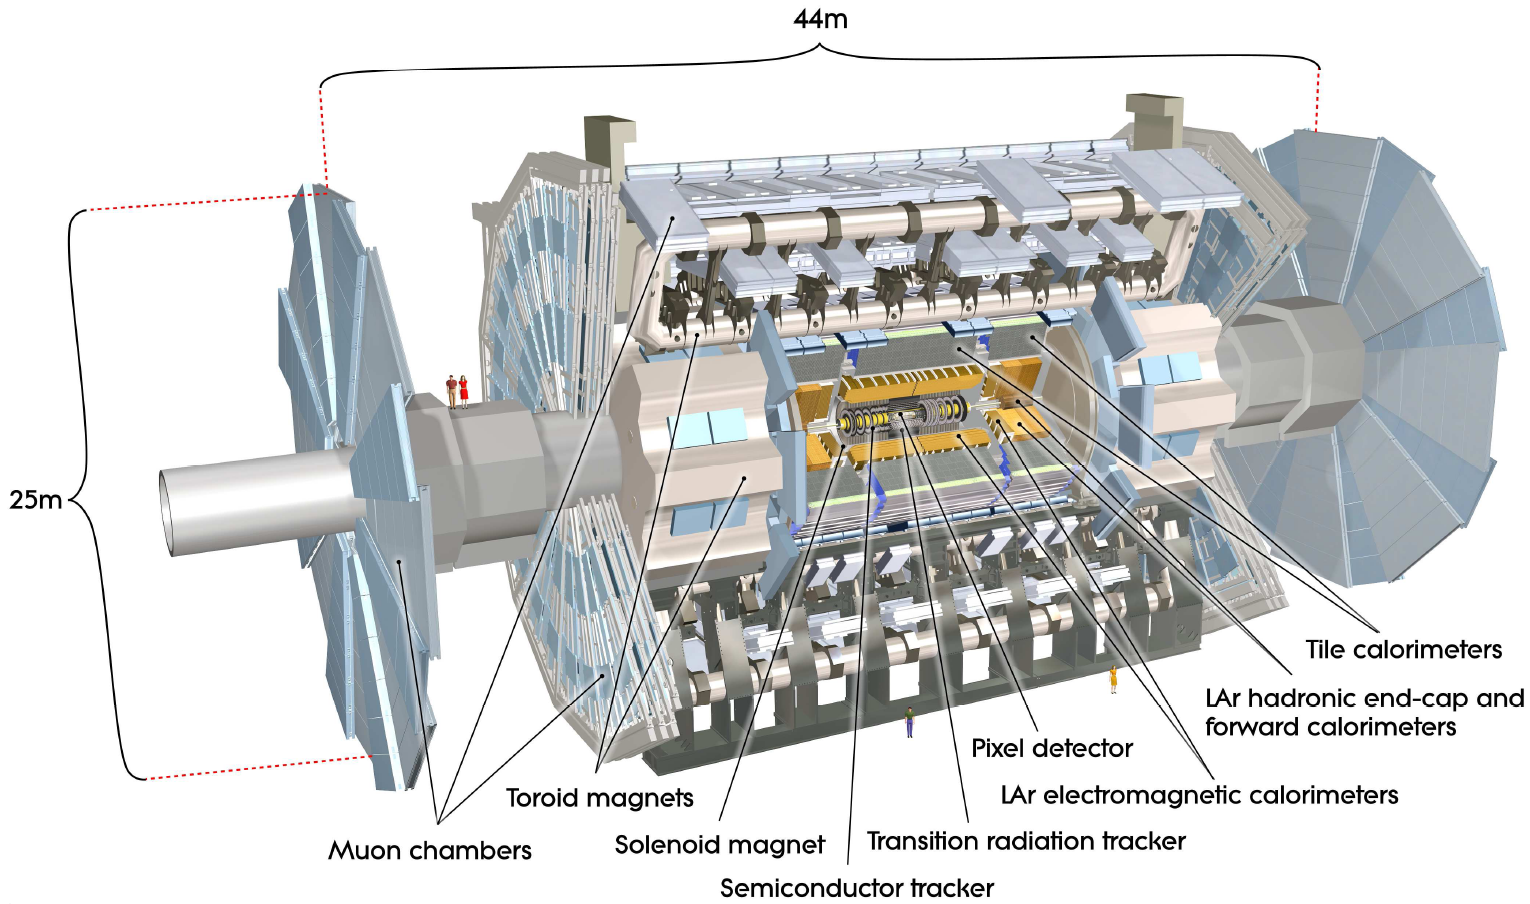
\includegraphics[width=0.85\textwidth]{p1-figs/atlas.png}
				 	\end{figure}

          \vspace{-0.8cm}
          \begin{figure}
						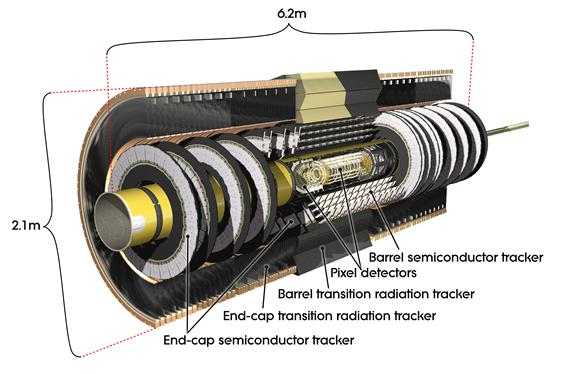
\includegraphics[width=0.85\textwidth]{p1-figs/id.jpg}
				 	\end{figure}

        \end{column}
        \end{columns}

    }

    \subsection{HL-LHC \& ITk}


    % ============================================================== %
    %
    % HL-LHC & ITK Frame
    %
    % ============================================================== %

    \frame{
      \frametitle{High Luminosity LHC \& ITk Upgrades}
      %

        \begin{columns}[T,onlytextwidth]
        \begin{column}{.54\textwidth}

        \begin{block}{ $3x$ increase in instantaneous luminosity! }
            \begin{itemize}
              \item $L = $\num{2e73} fb$^{-1}$ s$^{-1} \rightarrow
                     L = $ \num{7e73} fb$^{-1}$ s$^{-1} $ \\
            \end{itemize}
          \end{block}

        \end{column}
        \begin{column}{.4\textwidth}
				\vspace{-1.2cm}
					\begin{figure}
						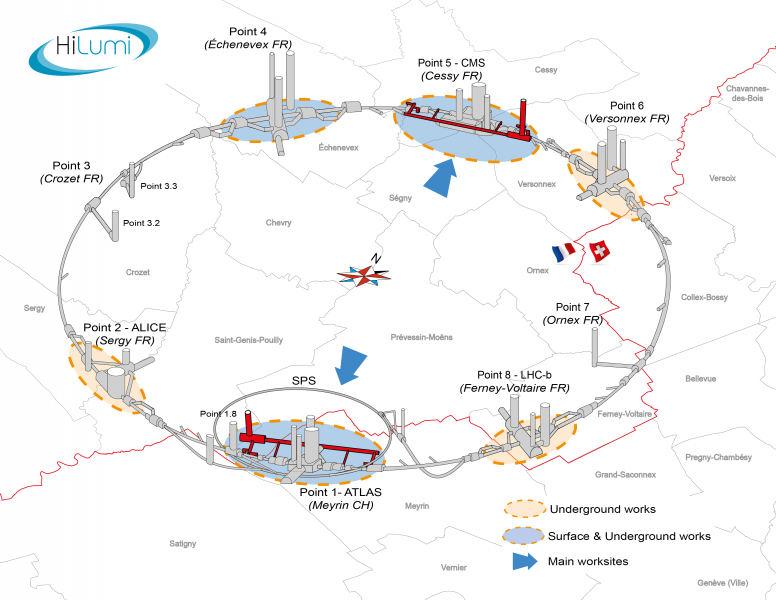
\includegraphics
						[width=\textwidth, height=.4\textheight]
						{p1-figs/hl-upgrade.png}
				 	\end{figure}

        \end{column}
        \end{columns}

        \vspace{-0.1cm}

        \begin{minipage}{\textwidth}
          \begin{columns}[T,onlytextwidth]
          \begin{column}{.5\textwidth}
            \begin{figure}
              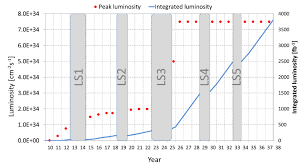
\includegraphics
              [height=.47\textheight]
              {p1-figs/hl.png}
            \end{figure}
          \end{column}
          \begin{column}{.6\textwidth}
            \vspace{0.5cm}
            \begin{figure}
              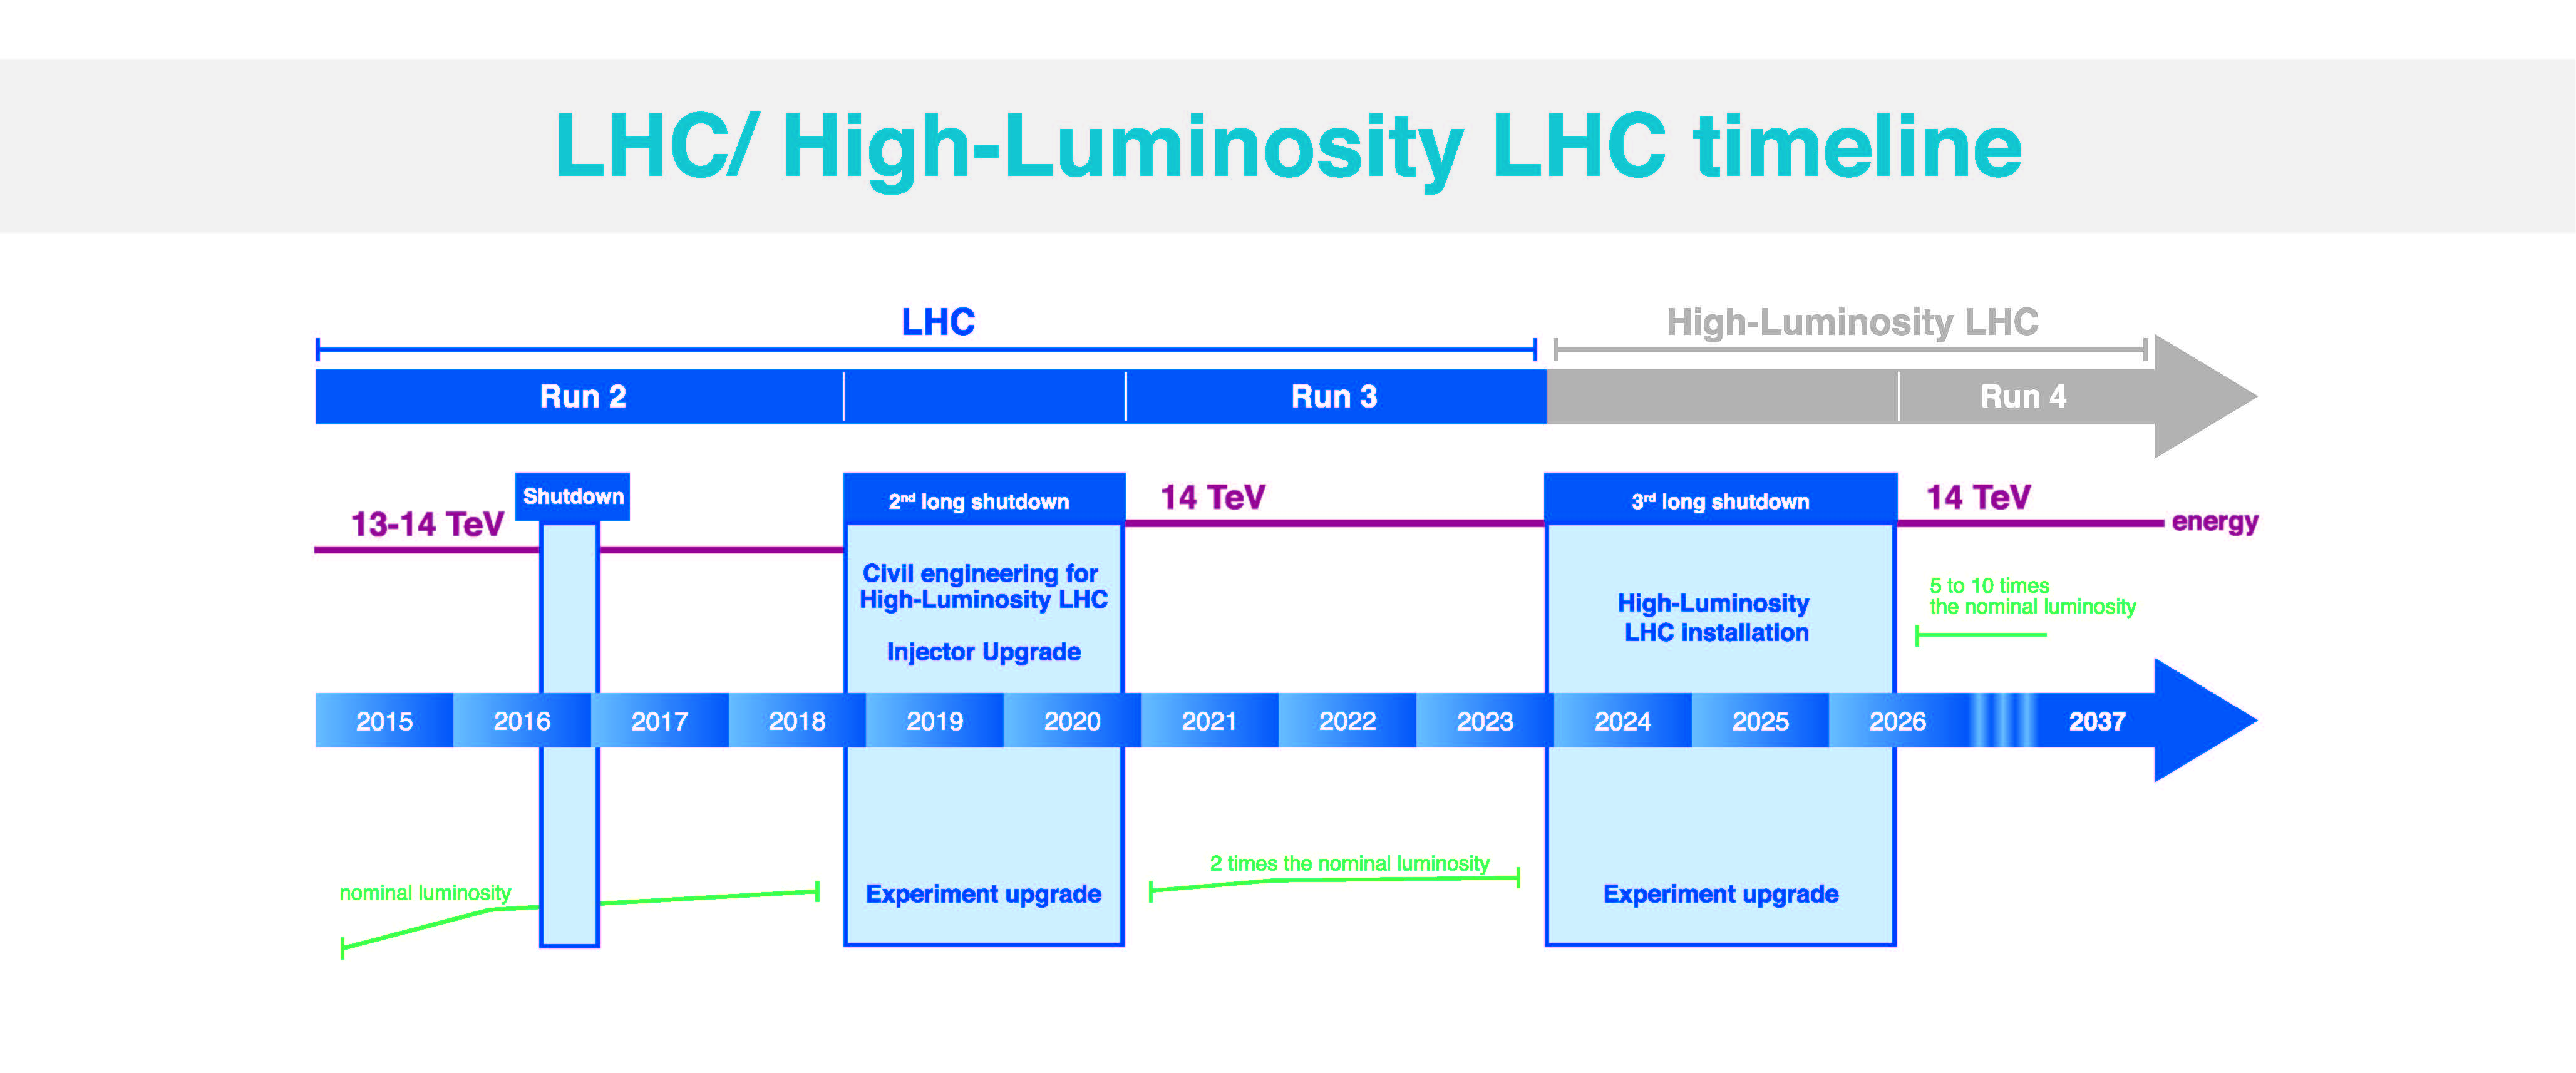
\includegraphics
              [scale=0.17,trim={6cm 1cm 6cm 6cm },clip=true]
              {p1-figs/hl-plan.jpg}
            \end{figure}
          \end{column}
          \end{columns}

        \end{minipage}

    }

    \frame{
      \frametitle{High Luminosity LHC \& ITk Upgrades}
      %

        \begin{columns}[T,onlytextwidth]
        \begin{column}{.54\textwidth}

        \begin{block}{ $3x$ increase in instantaneous luminosity! }
            \begin{itemize}
              \item $L = $\num{2e73} fb$^{-1}$ s$^{-1} \rightarrow
                     L = $ \num{7e73} fb$^{-1}$ s$^{-1} $ \\
              \item {\bf More particles, more problems}
            \end{itemize}
          \end{block}

        \end{column}
        \begin{column}{.4\textwidth}
				  \vspace{-1.2cm}
					\begin{figure}
						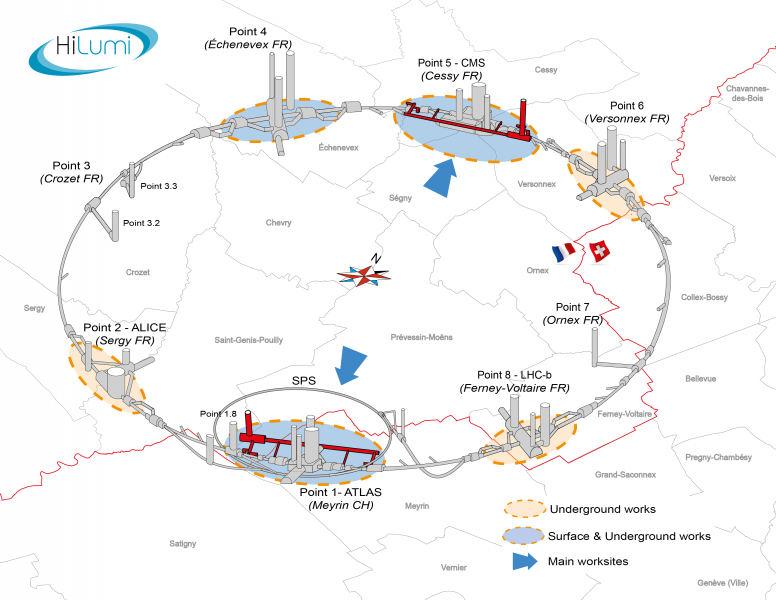
\includegraphics
						[width=\textwidth, height=.4\textheight]
						{p1-figs/hl-upgrade.png}
				 	\end{figure}

        \end{column}
        \end{columns}


        \begin{minipage}{\textwidth}
          \begin{columns}[T,onlytextwidth]
          \begin{column}{.5\textwidth}
            \begin{figure}
              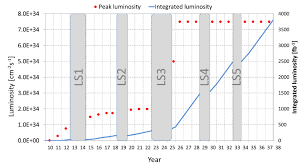
\includegraphics
              [height=.47\textheight]
              {p1-figs/hl.png}
            \end{figure}
          \end{column}
          \begin{column}{.6\textwidth}
            \vspace{0.5cm}
            \begin{figure}
              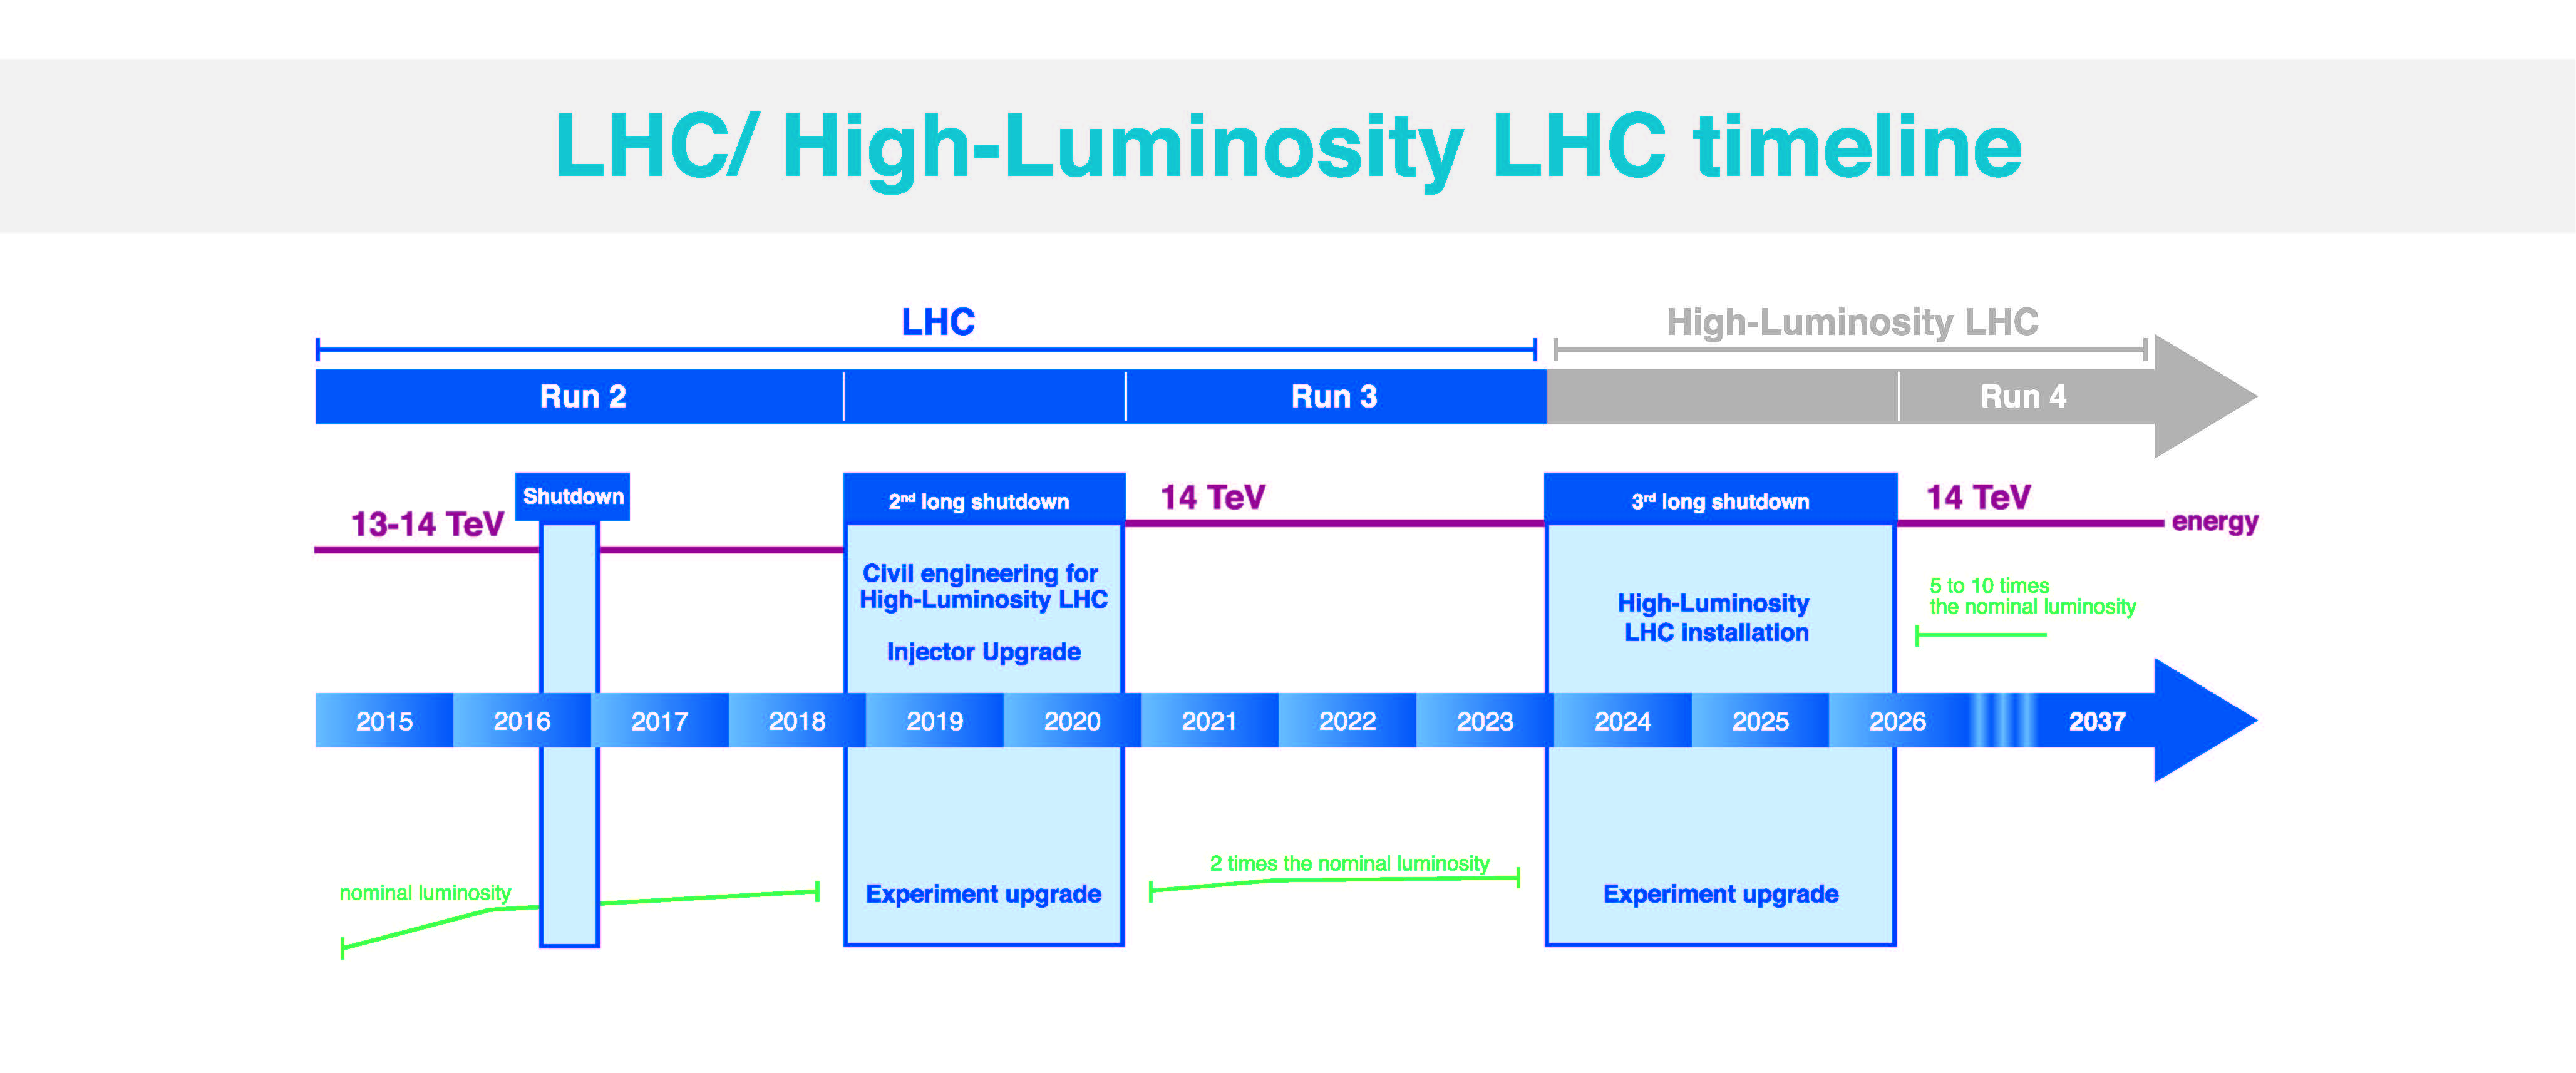
\includegraphics
              [scale=0.17,trim={6cm 1cm 6cm 6cm },clip=true]
              {p1-figs/hl-plan.jpg}
            \end{figure}
          \end{column}
          \end{columns}

        \end{minipage}

    }

    \frame{
      \frametitle{High Luminosity LHC \& ITk Upgrades}
      %

        \begin{columns}[T,onlytextwidth]
        \begin{column}{.54\textwidth}

        \begin{block}{ $3x$ increase in instantaneous luminosity! }
            \begin{itemize}
              \item $L = $\num{2e73} fb$^{-1}$ s$^{-1} \rightarrow
                     L = $ \num{7e73} fb$^{-1}$ s$^{-1} $ \\
            \end{itemize}
          \end{block}

        \end{column}
        \begin{column}{.4\textwidth}
				\vspace{-1.2cm}
					\begin{figure}
						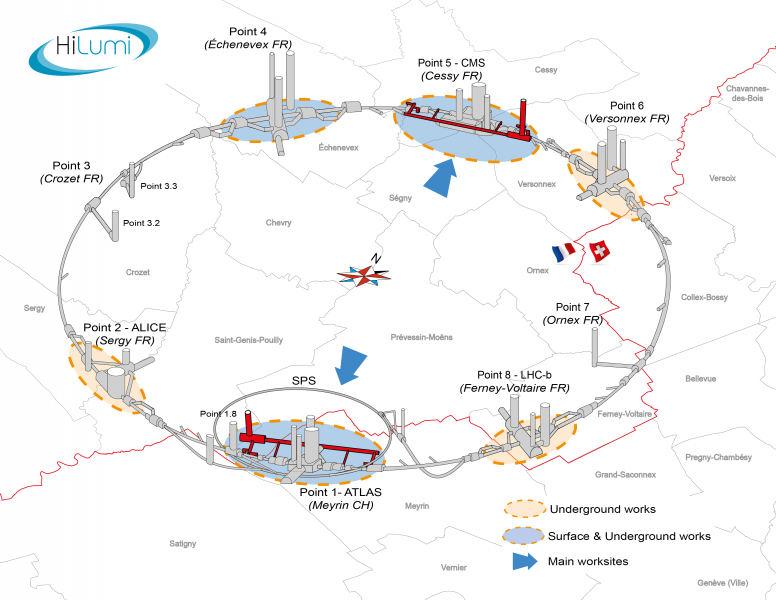
\includegraphics
						[width=\textwidth, height=.4\textheight]
						{p1-figs/hl-upgrade.png}
				 	\end{figure}

        \end{column}
        \end{columns}

        \begin{minipage}{\textwidth}
          \begin{block}{ The inner detector has insufficient:}
            \begin{itemize}
                \item radiation hardness
                \item granularity
                \item readout bandwidth
                \item trigger readout
            \end{itemize}
          \end{block}
        \end{minipage}

    }

    \frame{
      \frametitle{High Luminosity LHC \& ITk Upgrades}
      %

        \begin{columns}[T,onlytextwidth]
        \begin{column}{.54\textwidth}

        \begin{block}{ $3x$ increase in instantaneous luminosity! }
            \begin{itemize}
              \item $L = $\num{2e73} fb$^{-1}$ s$^{-1} \rightarrow
                     L = $ \num{7e73} fb$^{-1}$ s$^{-1} $ \\
            \end{itemize}
          \end{block}

        \end{column}
        \begin{column}{.4\textwidth}
				\vspace{-1.2cm}
					\begin{figure}
						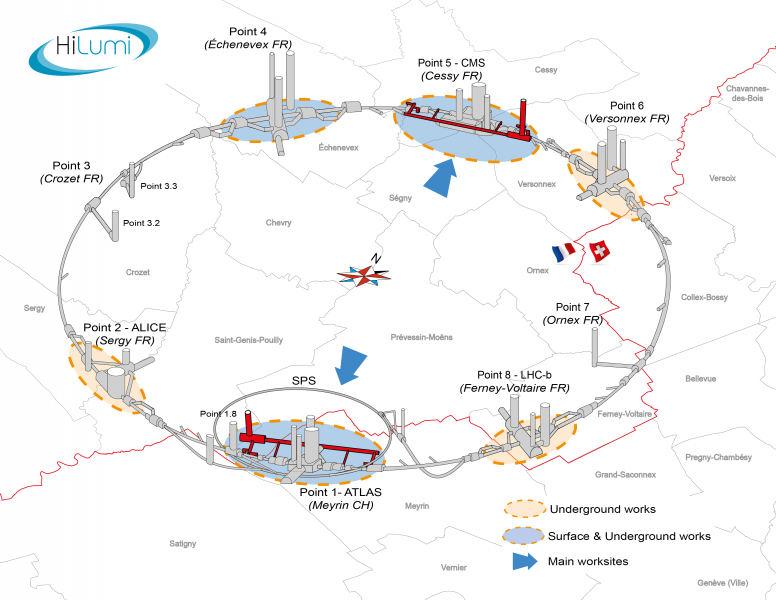
\includegraphics
						[width=\textwidth, height=.4\textheight]
						{p1-figs/hl-upgrade.png}
				 	\end{figure}

        \end{column}
        \end{columns}

        \begin{minipage}{\textwidth}
          \begin{block}{ The inner detector has insufficient:}
            \begin{itemize}
              \item radiation hardness: HL-LHC will deliver 4000 fb$^{-1}$  integrated luminosity,
                    ID PIX is designed for 400 fb$^{-1}$, ID SCT for 700 fb$^{-1}$,
                    IBL for 800 fb$^{-1}$
            \end{itemize}
          \end{block}
        \end{minipage}

    }

    \frame{
      \frametitle{High Luminosity LHC \& ITk Upgrades}
      %

        \begin{columns}[T,onlytextwidth]
        \begin{column}{.54\textwidth}

        \begin{block}{ $3x$ increase in instantaneous luminosity! }
            \begin{itemize}
              \item $L = $\num{2e73} fb$^{-1}$ s$^{-1} \rightarrow
                     L = $ \num{7e73} fb$^{-1}$ s$^{-1} $ \\
            \end{itemize}
          \end{block}

        \end{column}
        \begin{column}{.4\textwidth}
				\vspace{-1.2cm}
					\begin{figure}
						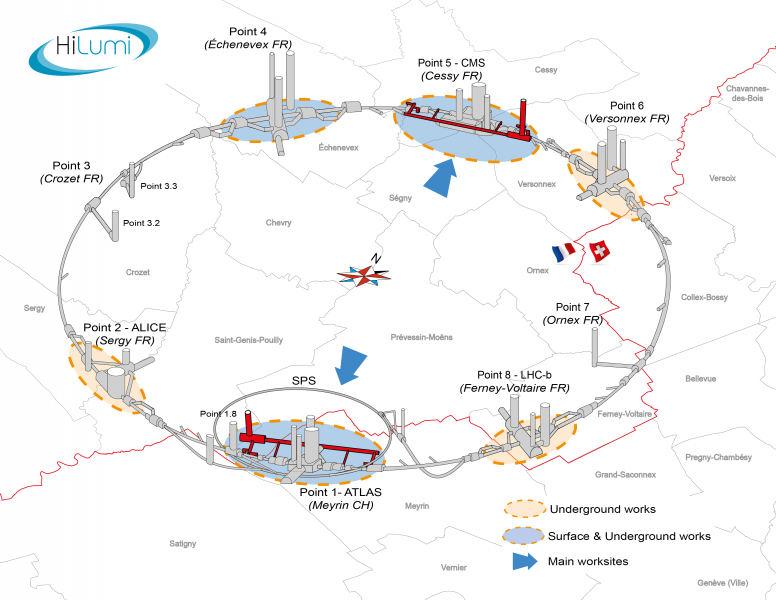
\includegraphics
						[width=\textwidth, height=.4\textheight]
						{p1-figs/hl-upgrade.png}
				 	\end{figure}

        \end{column}
        \end{columns}

        \begin{minipage}{\textwidth}
          \begin{block}{ The inner detector has insufficient:}
            \begin{itemize}
              \item granularity: Increasing fluence means higher granularity is needed to maintain performance; compensate for instrinsic dead time
                % -- in all detectors you have whats called dead time;
                %    in semiconducotr detectors, as charged particles stream through the
                %    semiconductor, it loses particles to valence electrons and promotes them
                %    to the conduction band, and, because of the bias voltage across the device they
                %    drift to the anode, where the signal is readout.
                %    If another particle enters the detector volume during the electron drift time,
                %    either you'll distort the output signal due to the pulses piling up, or youll
                %    miss the 2nd pulse entirely. To mitigate this loss/distortion of events,
                %    we make our detectors smaller and increase the number of readout channels
            \end{itemize}
          \end{block}
        \end{minipage}

    }

    \frame{
      \frametitle{High Luminosity LHC \& ITk Upgrades}
      %

        \begin{columns}[T,onlytextwidth]
        \begin{column}{.54\textwidth}

        \begin{block}{ $3x$ increase in instantaneous luminosity! }
            \begin{itemize}
              \item $L = $\num{2e73} fb$^{-1}$ s$^{-1} \rightarrow
                     L = $ \num{7e73} fb$^{-1}$ s$^{-1} $ \\
              \item \bf{More particles, more problems}
            \end{itemize}
          \end{block}

        \end{column}
        \begin{column}{.4\textwidth}
				\vspace{-1.2cm}
					\begin{figure}
						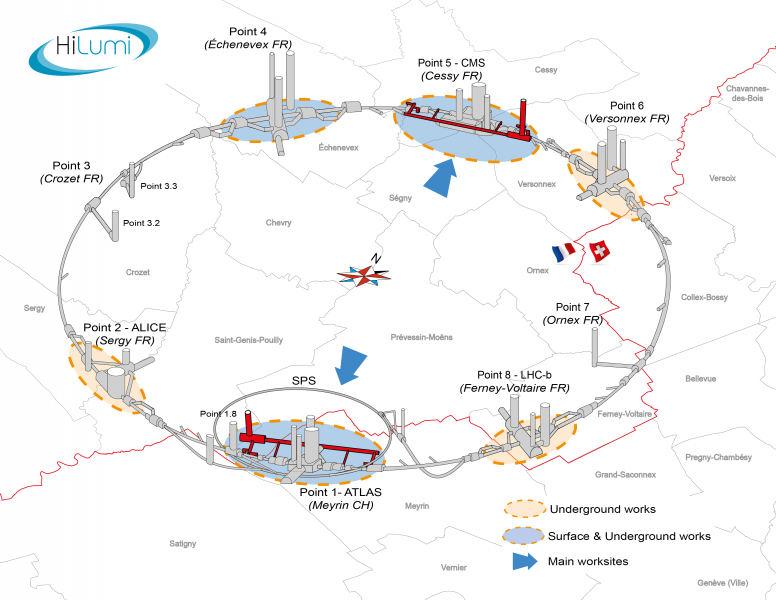
\includegraphics
						[width=\textwidth, height=.4\textheight]
						{p1-figs/hl-upgrade.png}
				 	\end{figure}

        \end{column}
        \end{columns}

        \begin{minipage}{\textwidth}
          \begin{block}{ The inner detector has insufficient:}
            \begin{itemize}
                \item readout bandwidth: HL-LHC will roughly quadruple ID designed bandwidth saturation
            \end{itemize}
          \end{block}
        \end{minipage}

    }

    \frame{
      \frametitle{High Luminosity LHC \& ITk Upgrades}
      %

        \begin{columns}[T,onlytextwidth]
        \begin{column}{.54\textwidth}

        \begin{block}{ $x10$ increase in instantaneous luminosity! }
            \begin{itemize}
              \item $L = $\num{1e73} fb$^{-1}$ s$^{-1} \rightarrow
                     L = $ \num{1e74} fb$^{-1}$ s$^{-1} $ \\
              \item \bf{More particles, more problems}
            \end{itemize}
          \end{block}

        \end{column}
        \begin{column}{.4\textwidth}
				\vspace{-1.2cm}
					\begin{figure}
						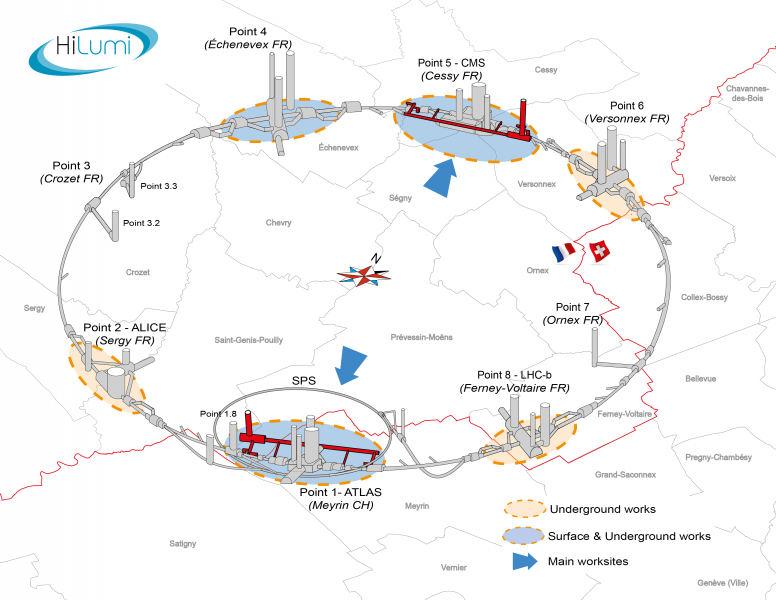
\includegraphics
						[width=\textwidth, height=.4\textheight]
						{p1-figs/hl-upgrade.png}
				 	\end{figure}

        \end{column}
        \end{columns}

        \begin{minipage}{\textwidth}
          \begin{block}{ The inner detector has insufficient:}
            \begin{itemize}
              \item trigger readout: readout chain must accomadate much higher hardware (level 1) trigger rate, and ideally include tracking info
            \end{itemize}
          \end{block}
        \end{minipage}

    }

    \frame{
      \frametitle{High Luminosity LHC \& ITk Upgrades}
      %

        \begin{columns}[T,onlytextwidth]
        \begin{column}{.54\textwidth}

        \begin{block}{ $x10$ increase in instantaneous luminosity! }
            \begin{itemize}
              \item $L = $\num{1e73} fb$^{-1}$ s$^{-1} \rightarrow
                     L = $ \num{1e74} fb$^{-1}$ s$^{-1} $ \\
              \item \bf{More particles, more problems}
            \end{itemize}
          \end{block}

        \end{column}
        \begin{column}{.4\textwidth}
				\vspace{-1.2cm}
					\begin{figure}
						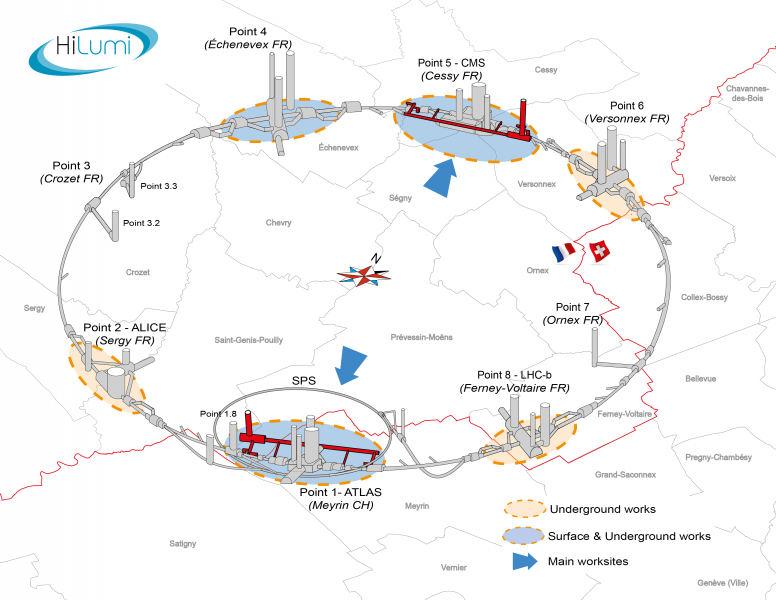
\includegraphics
						[width=\textwidth, height=.4\textheight]
						{p1-figs/hl-upgrade.png}
				 	\end{figure}

        \end{column}
        \end{columns}

        \begin{minipage}{\textwidth}
          \begin{block}{\large{\bf{Goal of ITk:}} }
            \large{\bf{Same or better performance than ID in
            harsh environment of HL-LHC}}
          \end{block}
        \end{minipage}
    }

    \subsection{ITk Design and Readout}

    \frame{ \frametitle{ITk design}
    \vspace{-0.2cm}
    \begin{minipage}{\textwidth}
    \begin{itemize}
      \item Pixel detector: 600M channels (80M in PIX): 5 barrel layers, encap system
      \item Strip detector: 70M channels (6M in SCT): 4 barrel layers, 6 EC rings
    \end{itemize}
    \end{minipage}
    \vspace{-0.1cm}

    \begin{minipage}{\textwidth}

        % design
				\begin{figure}
					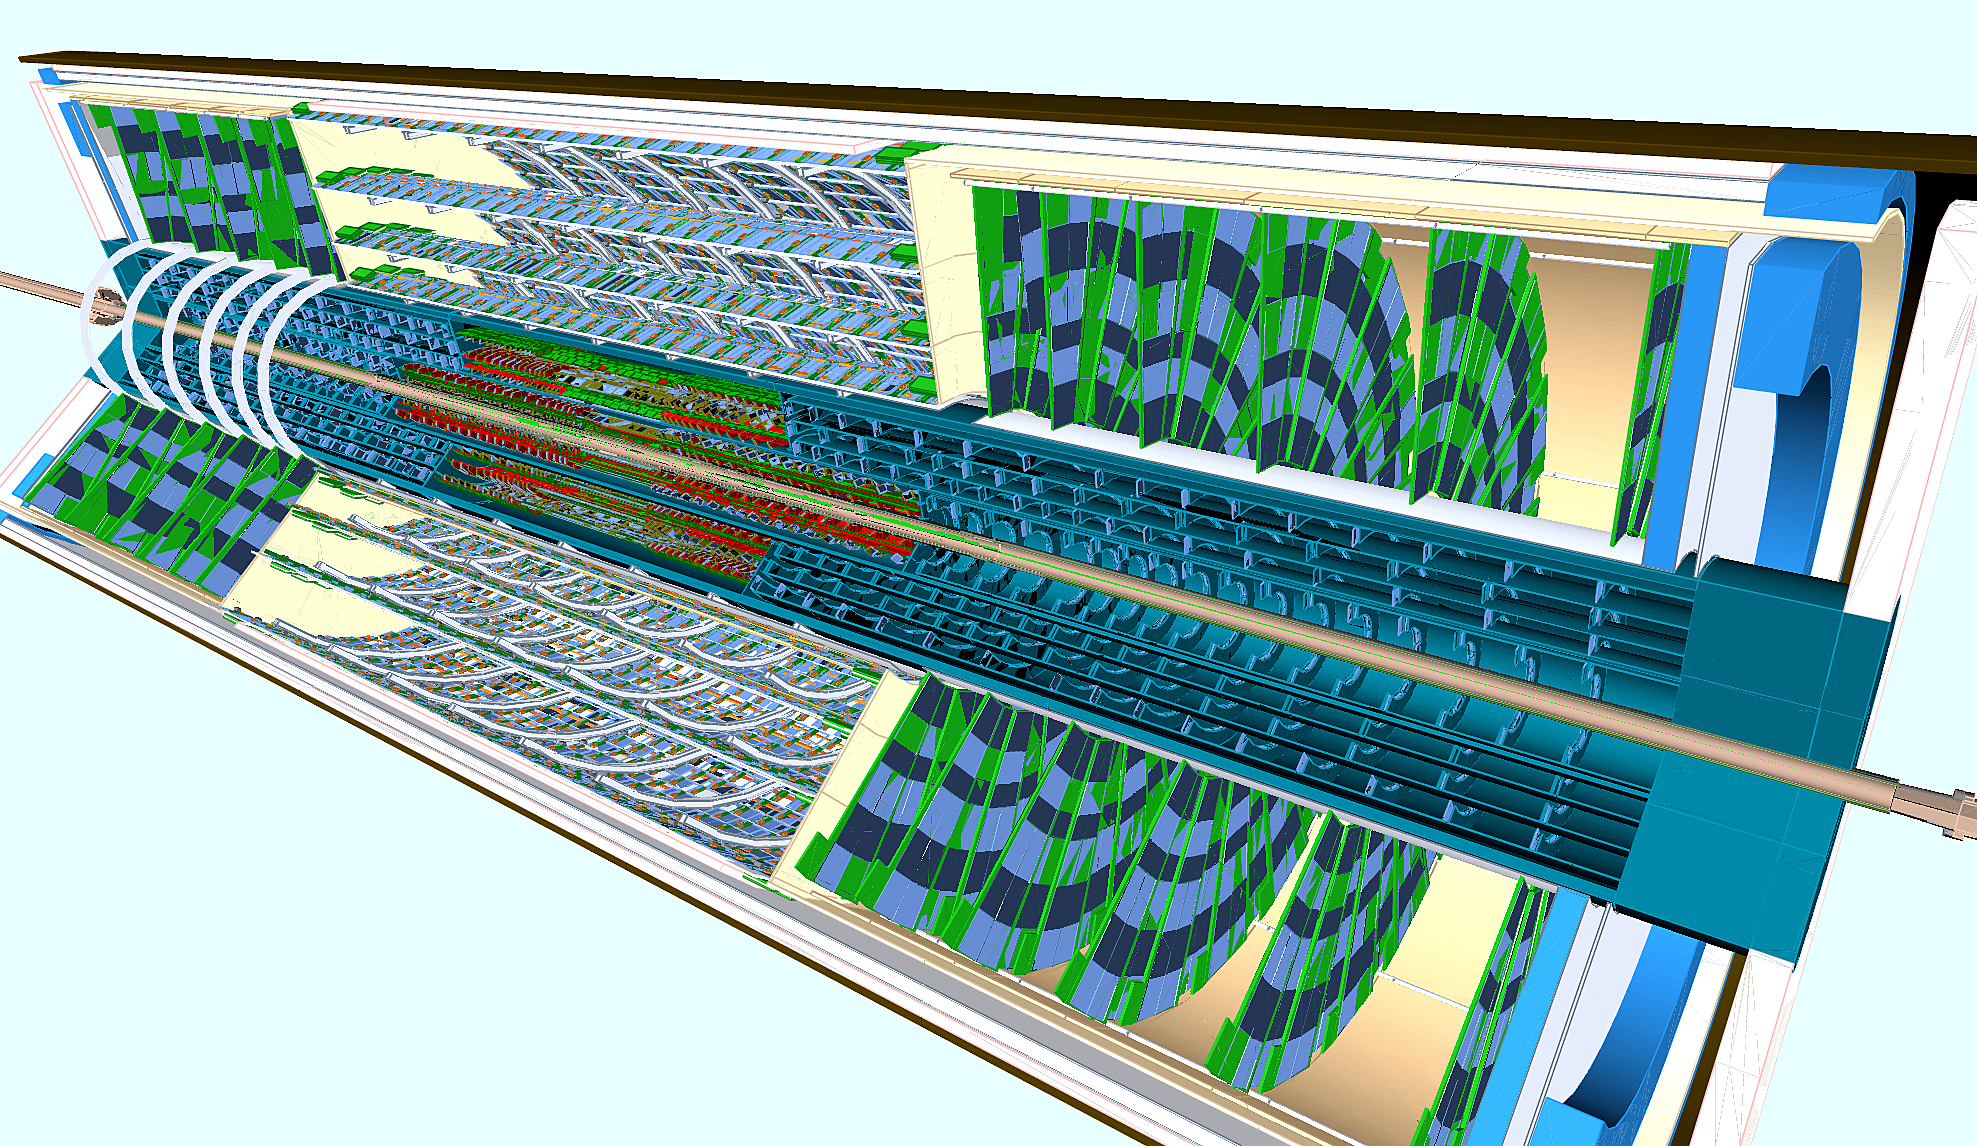
\includegraphics[trim={0cm 0cm 0cm 0cm},clip,width=0.7\textwidth ]{p1-figs/ATLASITK.png}
			 	\end{figure}

    \end{minipage}
    }


    \frame{
      \frametitle{ITk Strip Detector}
      % ignoring pixel detector
          \begin{itemize}
              \item Stave/petal: structure, cooling, power, electrical, etc.
              \item Module: silicon sensor + ASIC + readout hybrid + power board
              \item Hybrid: Flexible PCB with Hybrid Controller Chip (HCC) to interface w/ ASIC
          \end{itemize}

          \vspace{-0.4cm}

					\begin{figure}
						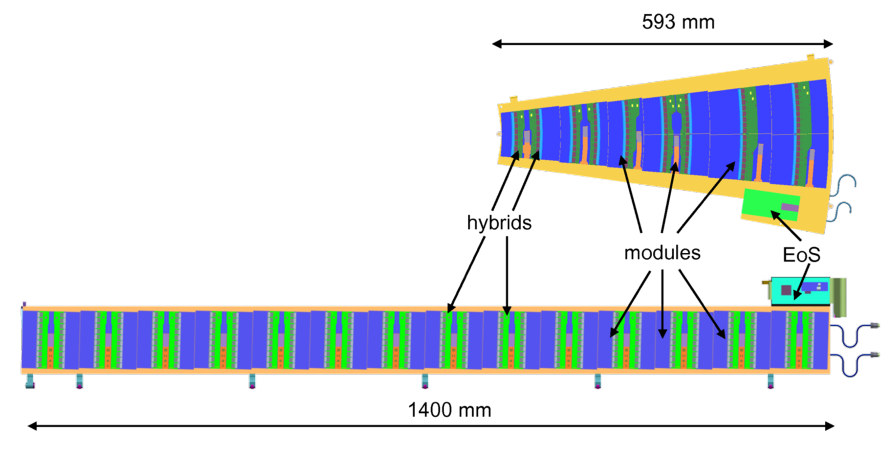
\includegraphics[trim={0cm 0cm 0cm 0cm},clip,width=0.8\textwidth]{p1-figs/stave_petal.png}
				 	\end{figure}

    }

    \frame{
      \frametitle{ITk Strip Detector Readout}
      % ignoring pixel detector
        \vspace{-0.2cm}
        \begin{itemize}
          \item sensor $\rightarrow$ front-end ASIC for signal amplification
            shaping, \& discrimination
          \item 10-12 ABC ASICs per hybrid; each ASIC reads out 256 ch
          \item Hybrid Controller Chip interfaces the stave/petal service bus \& front-end ASICs
        \end{itemize}
        \vspace{-0.2cm}

				\begin{figure}
					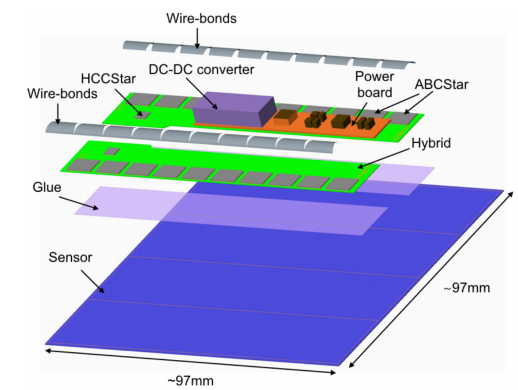
\includegraphics[trim={0cm 0cm 0cm 0cm},clip,width=0.5\textwidth]{p1-figs/module.png}
				\end{figure}

    }



    % ============================================================== %
    %
    % Our Progress
    %
    % ============================================================== %

    \section{Lab Testing of Hybrid Chips}
    \subsection{Testing Setup}

    \frame{
        \frametitle{Our Setup}
        \begin{columns}[c]
            \column{0.75\textwidth}
            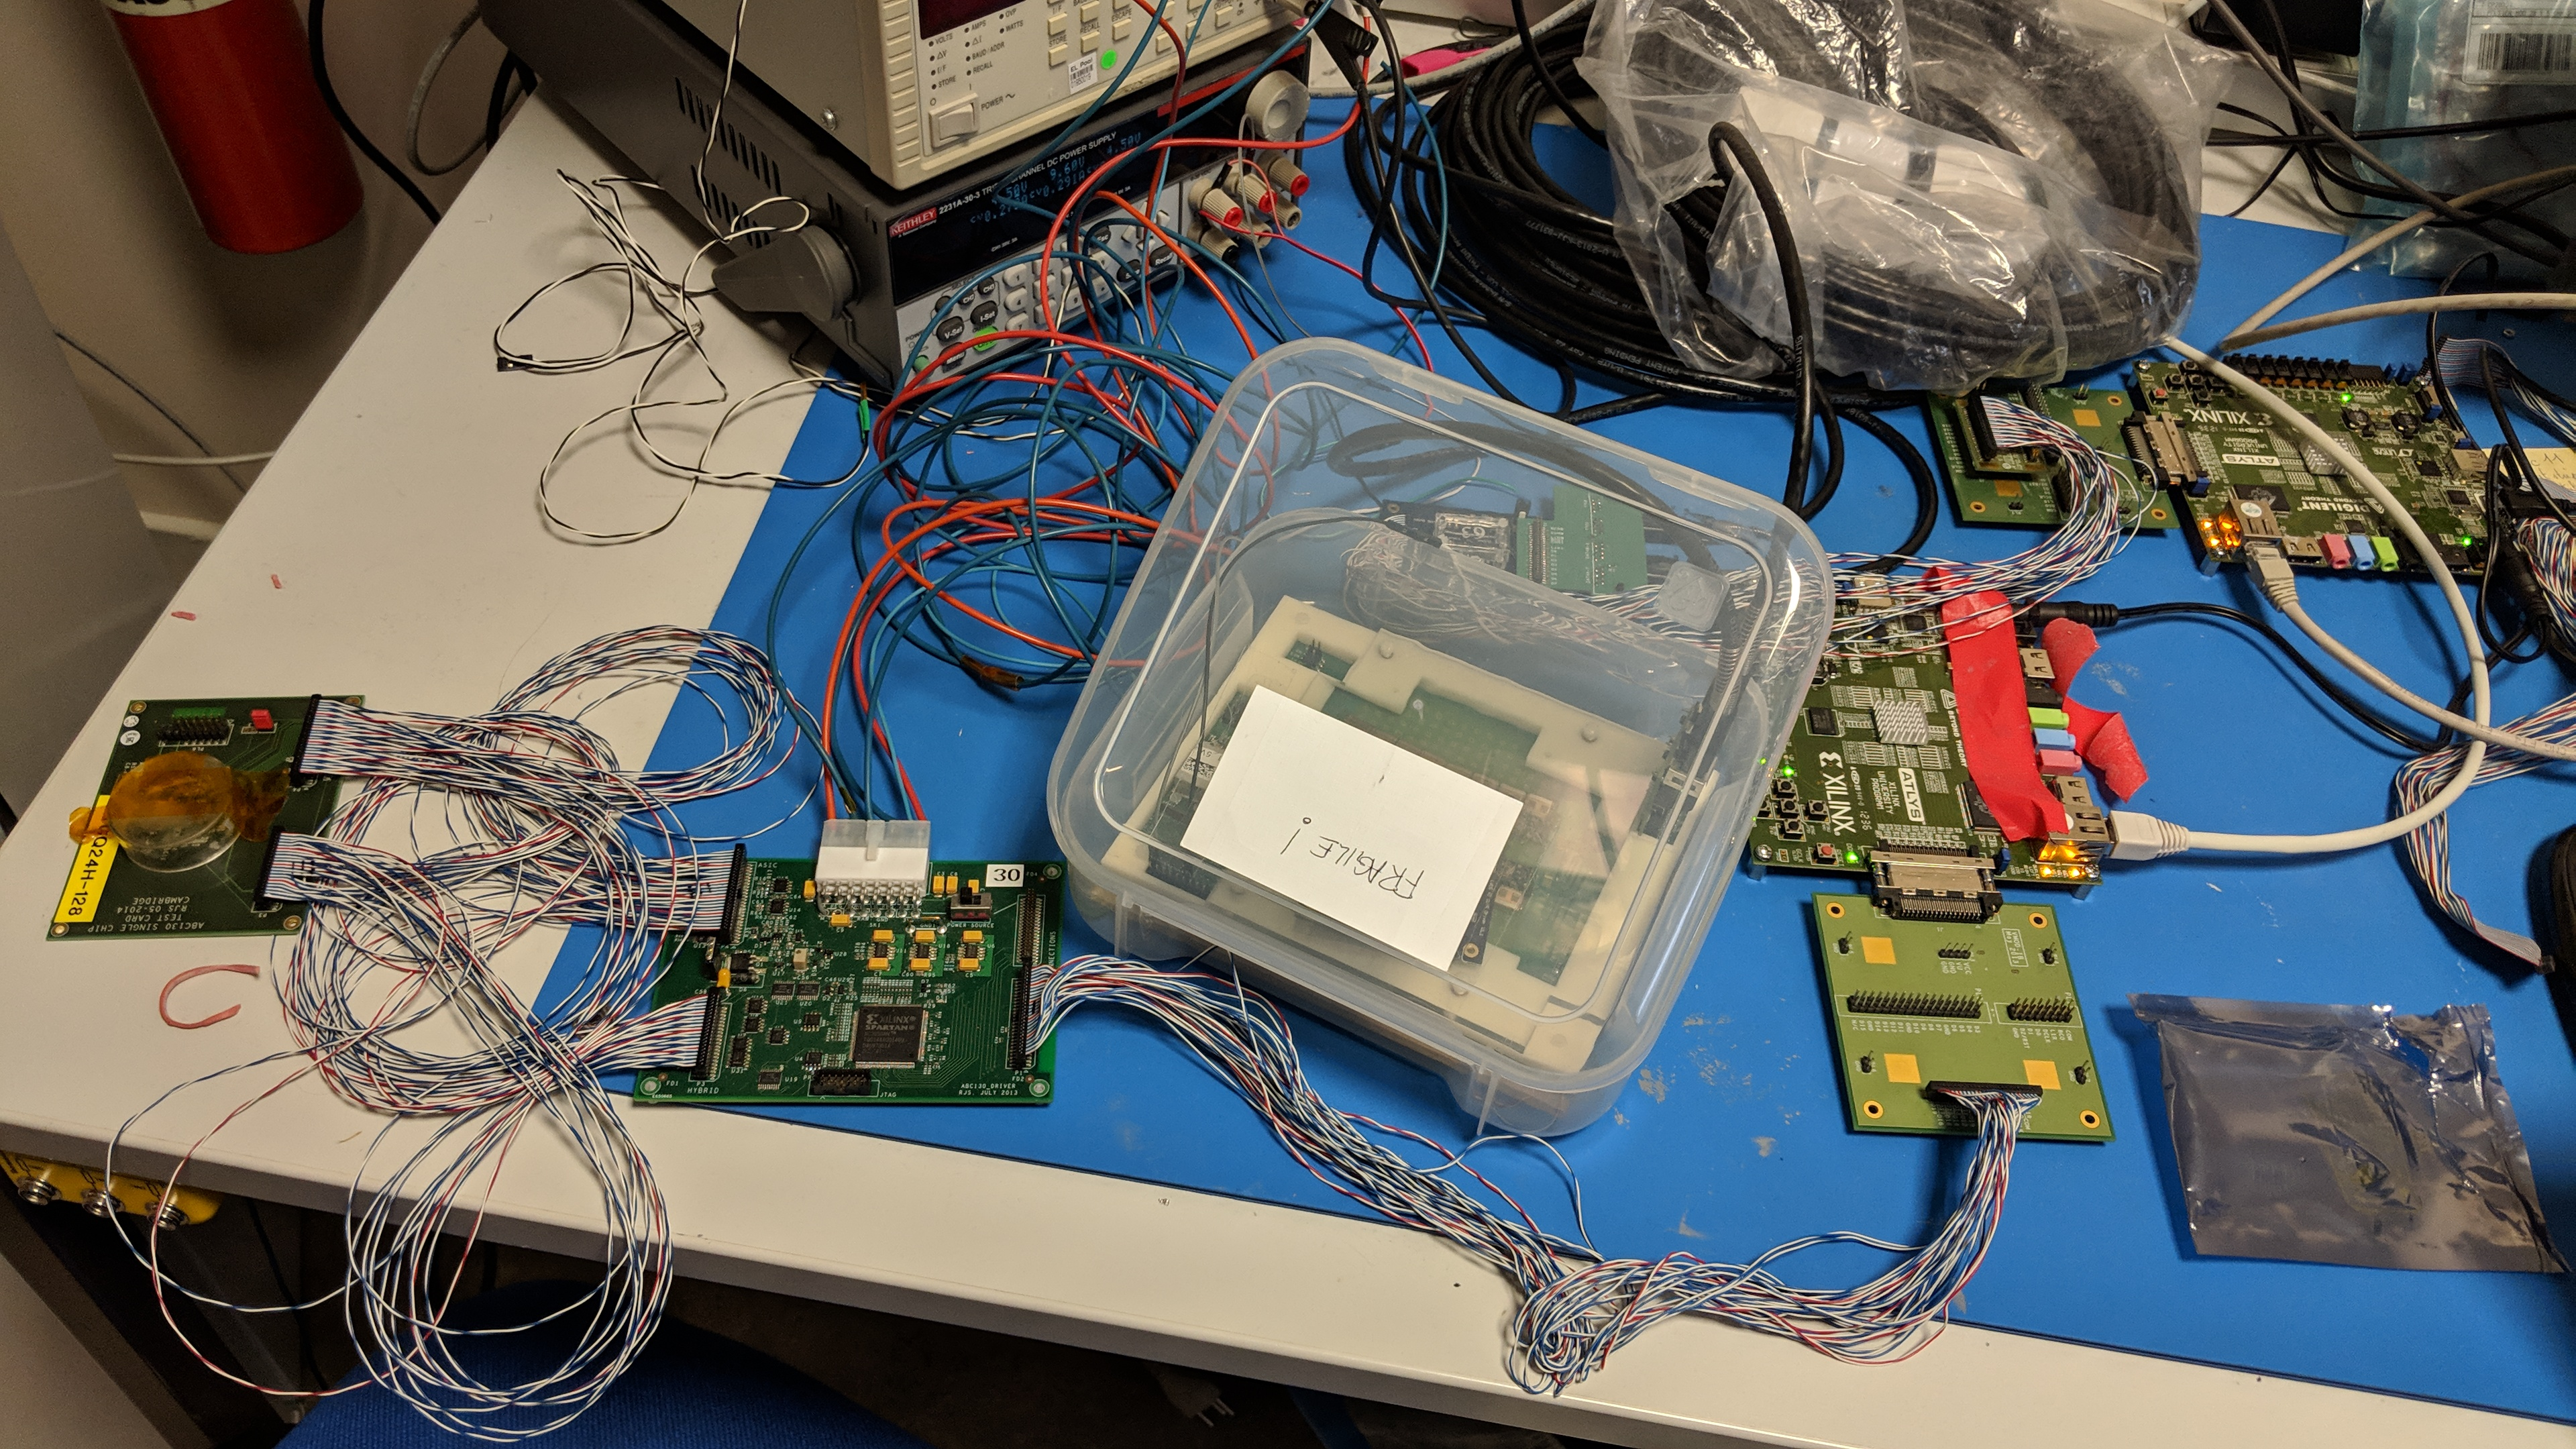
\includegraphics[width=1.0\textwidth]{images/whole_setup.jpg}

            \column{0.25\textwidth}
            \begin{block}{}
                Simple but elegant.
            \end{block}
        \end{columns}
    }

    \frame{
        \frametitle{Current DAQ Readout Chain}
        \begin{columns}[c]
            \column{0.75\textwidth}
            \includegraphics[width=1.0\textwidth]{images/readout_chain.jpg}

            \column{0.25\textwidth}
            \begin{block}{}
                A look at the fully assembled single chip readout chain, ending in the ABC130 prototype test board.
            \end{block}
        \end{columns}
    }

    \frame{
        \frametitle{ATLYS Board}
        \begin{columns}[c]
            \column{0.5\textwidth}
            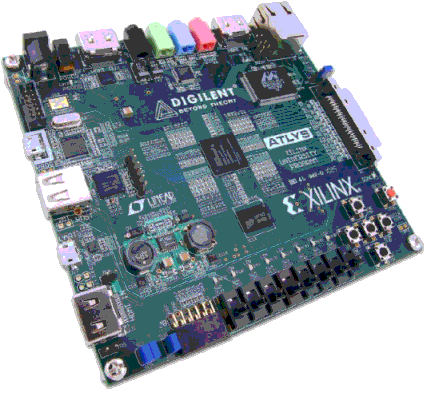
\includegraphics[width=1.0\textwidth]{images/atlys_pic.png}

            \column{0.5\textwidth}
            \begin{block}{}
                ATLYS is a low cost, widely available board that supports single chip, hybrid, and module tests.
            \end{block}
        \end{columns}
    }

    \frame{
        \frametitle{Interface Connection}
        \begin{columns}[c]
            \column{0.7\textwidth}
            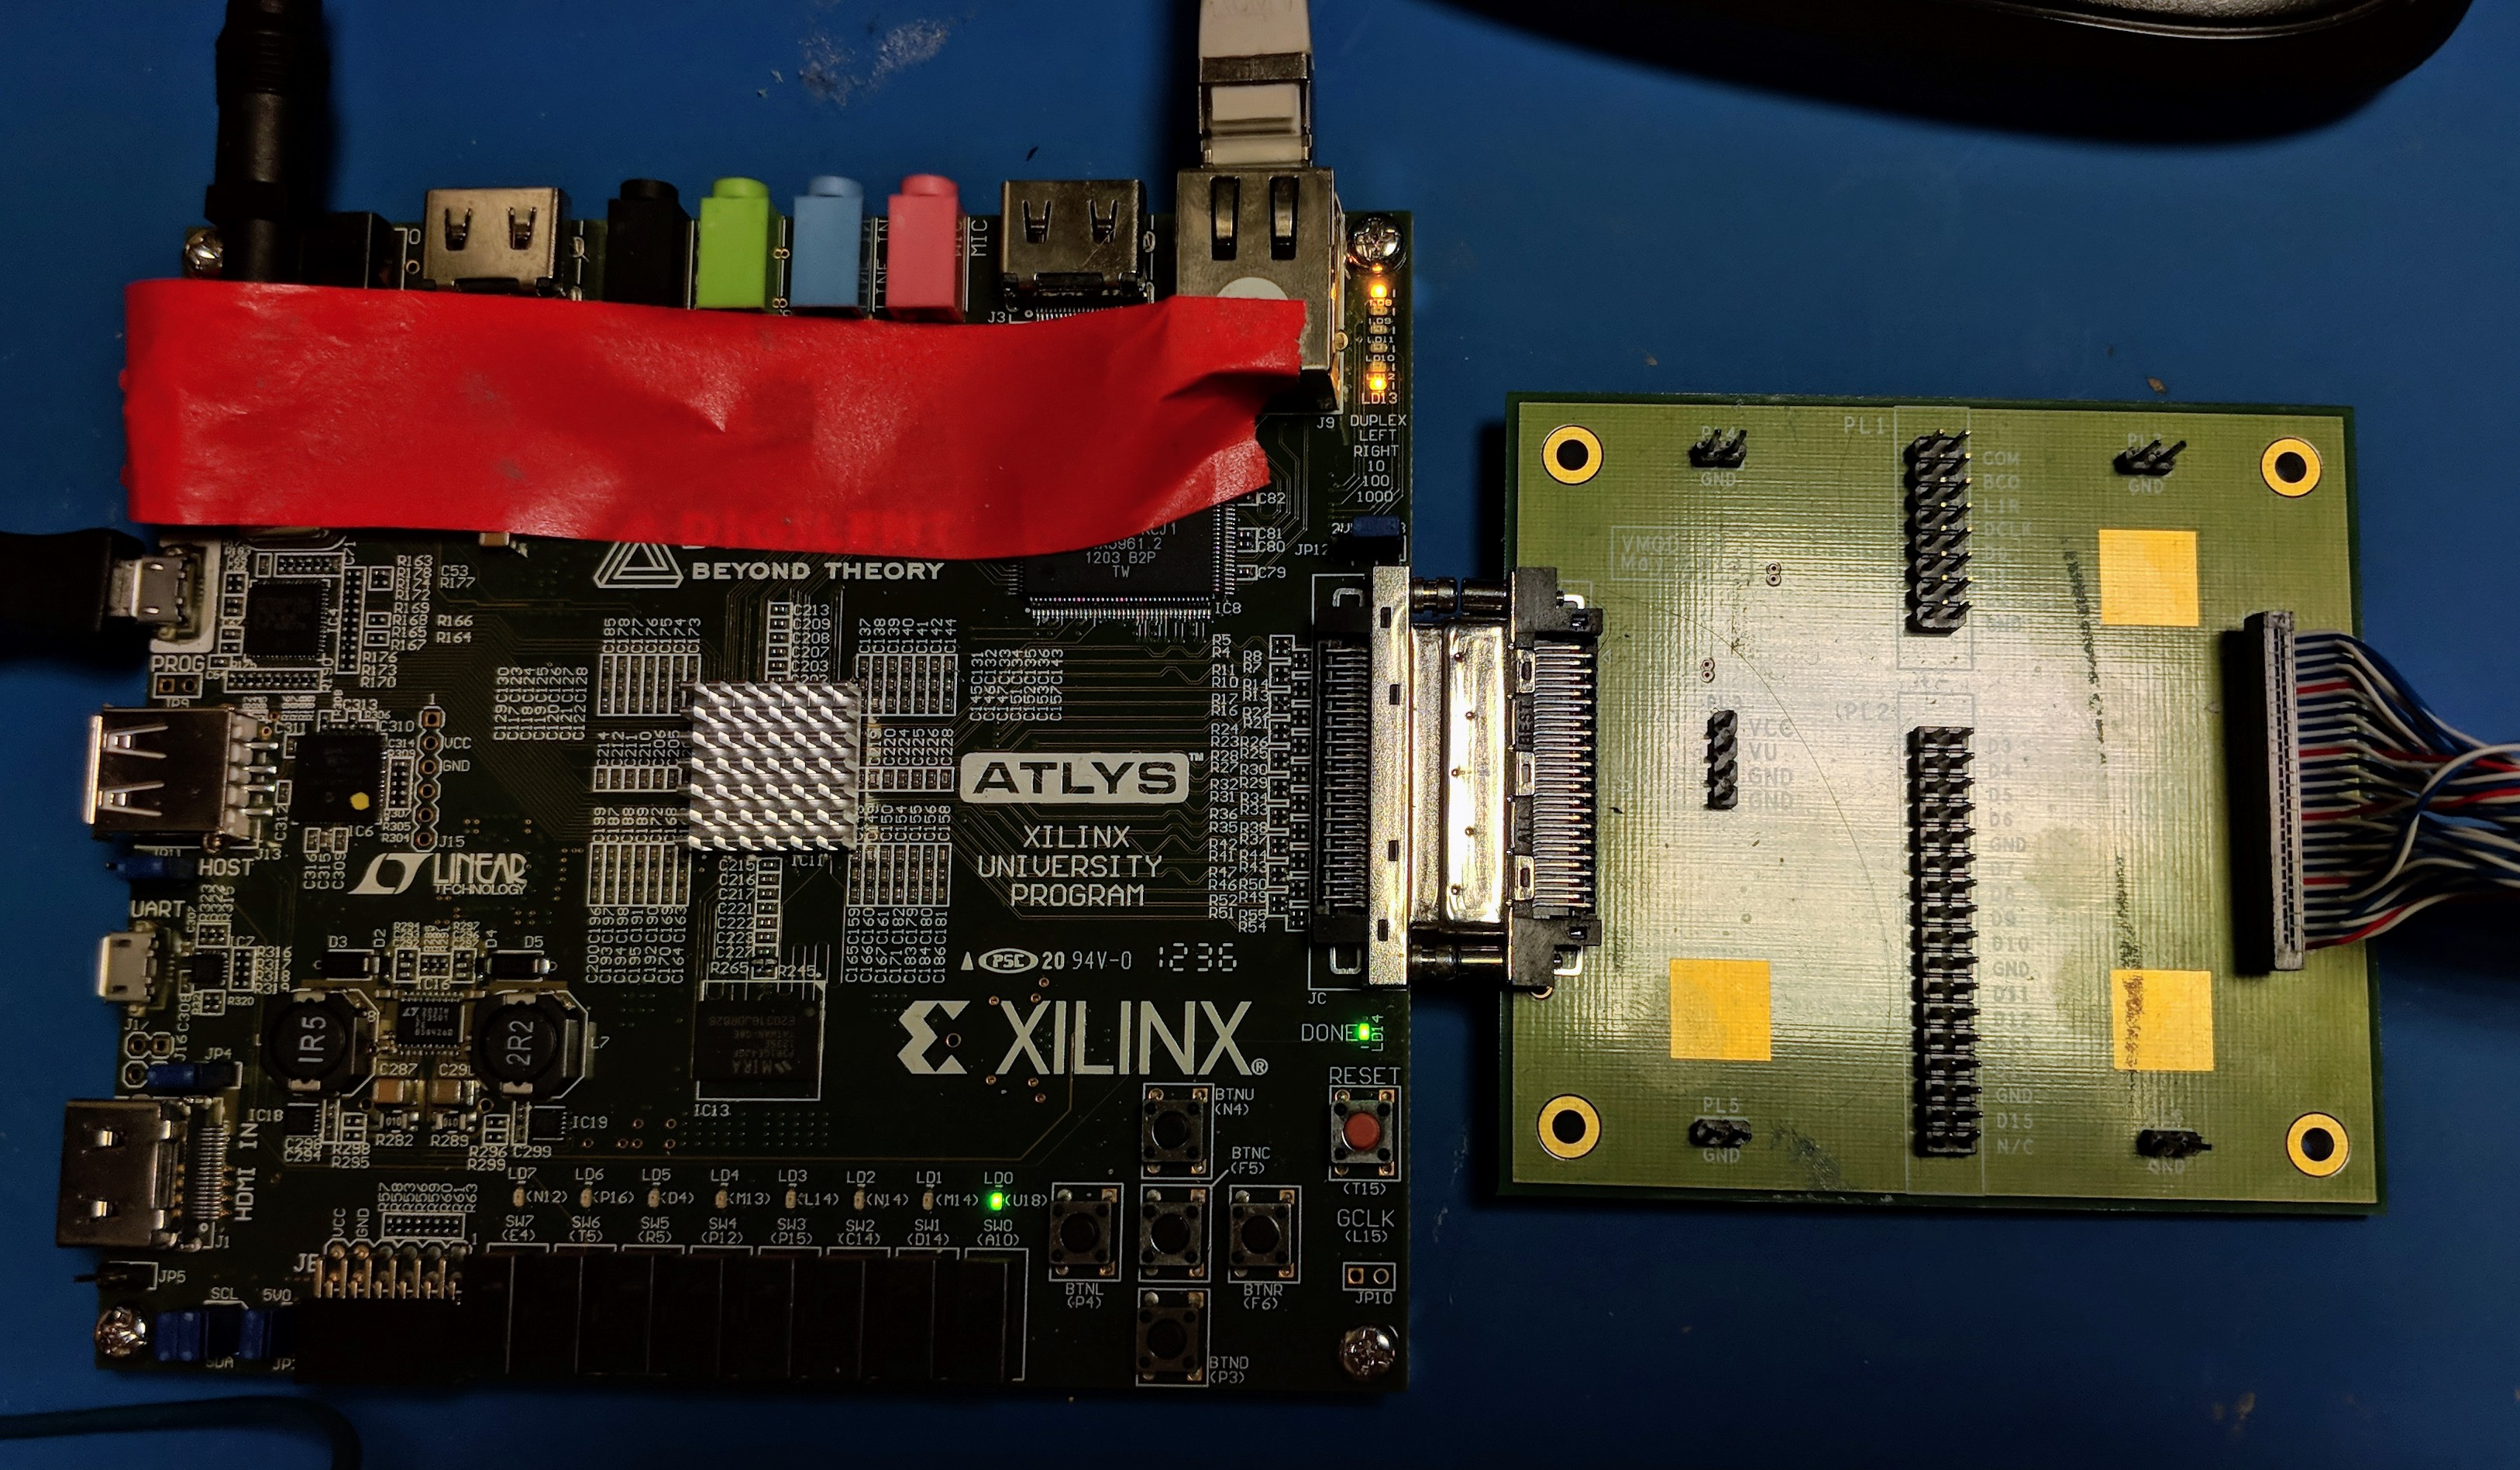
\includegraphics[width=1.0\textwidth]{images/ATLYSwithVMOD-IB.jpg}

            \column{0.3\textwidth}
            \begin{block}{}
                The ATLYS board is connected to to its interface board, VMOD-IB.
            \end{block}
        \end{columns}
    }

    \frame{
        \frametitle{Driver Board}
        \begin{columns}[c]
            \column{0.7\textwidth}
            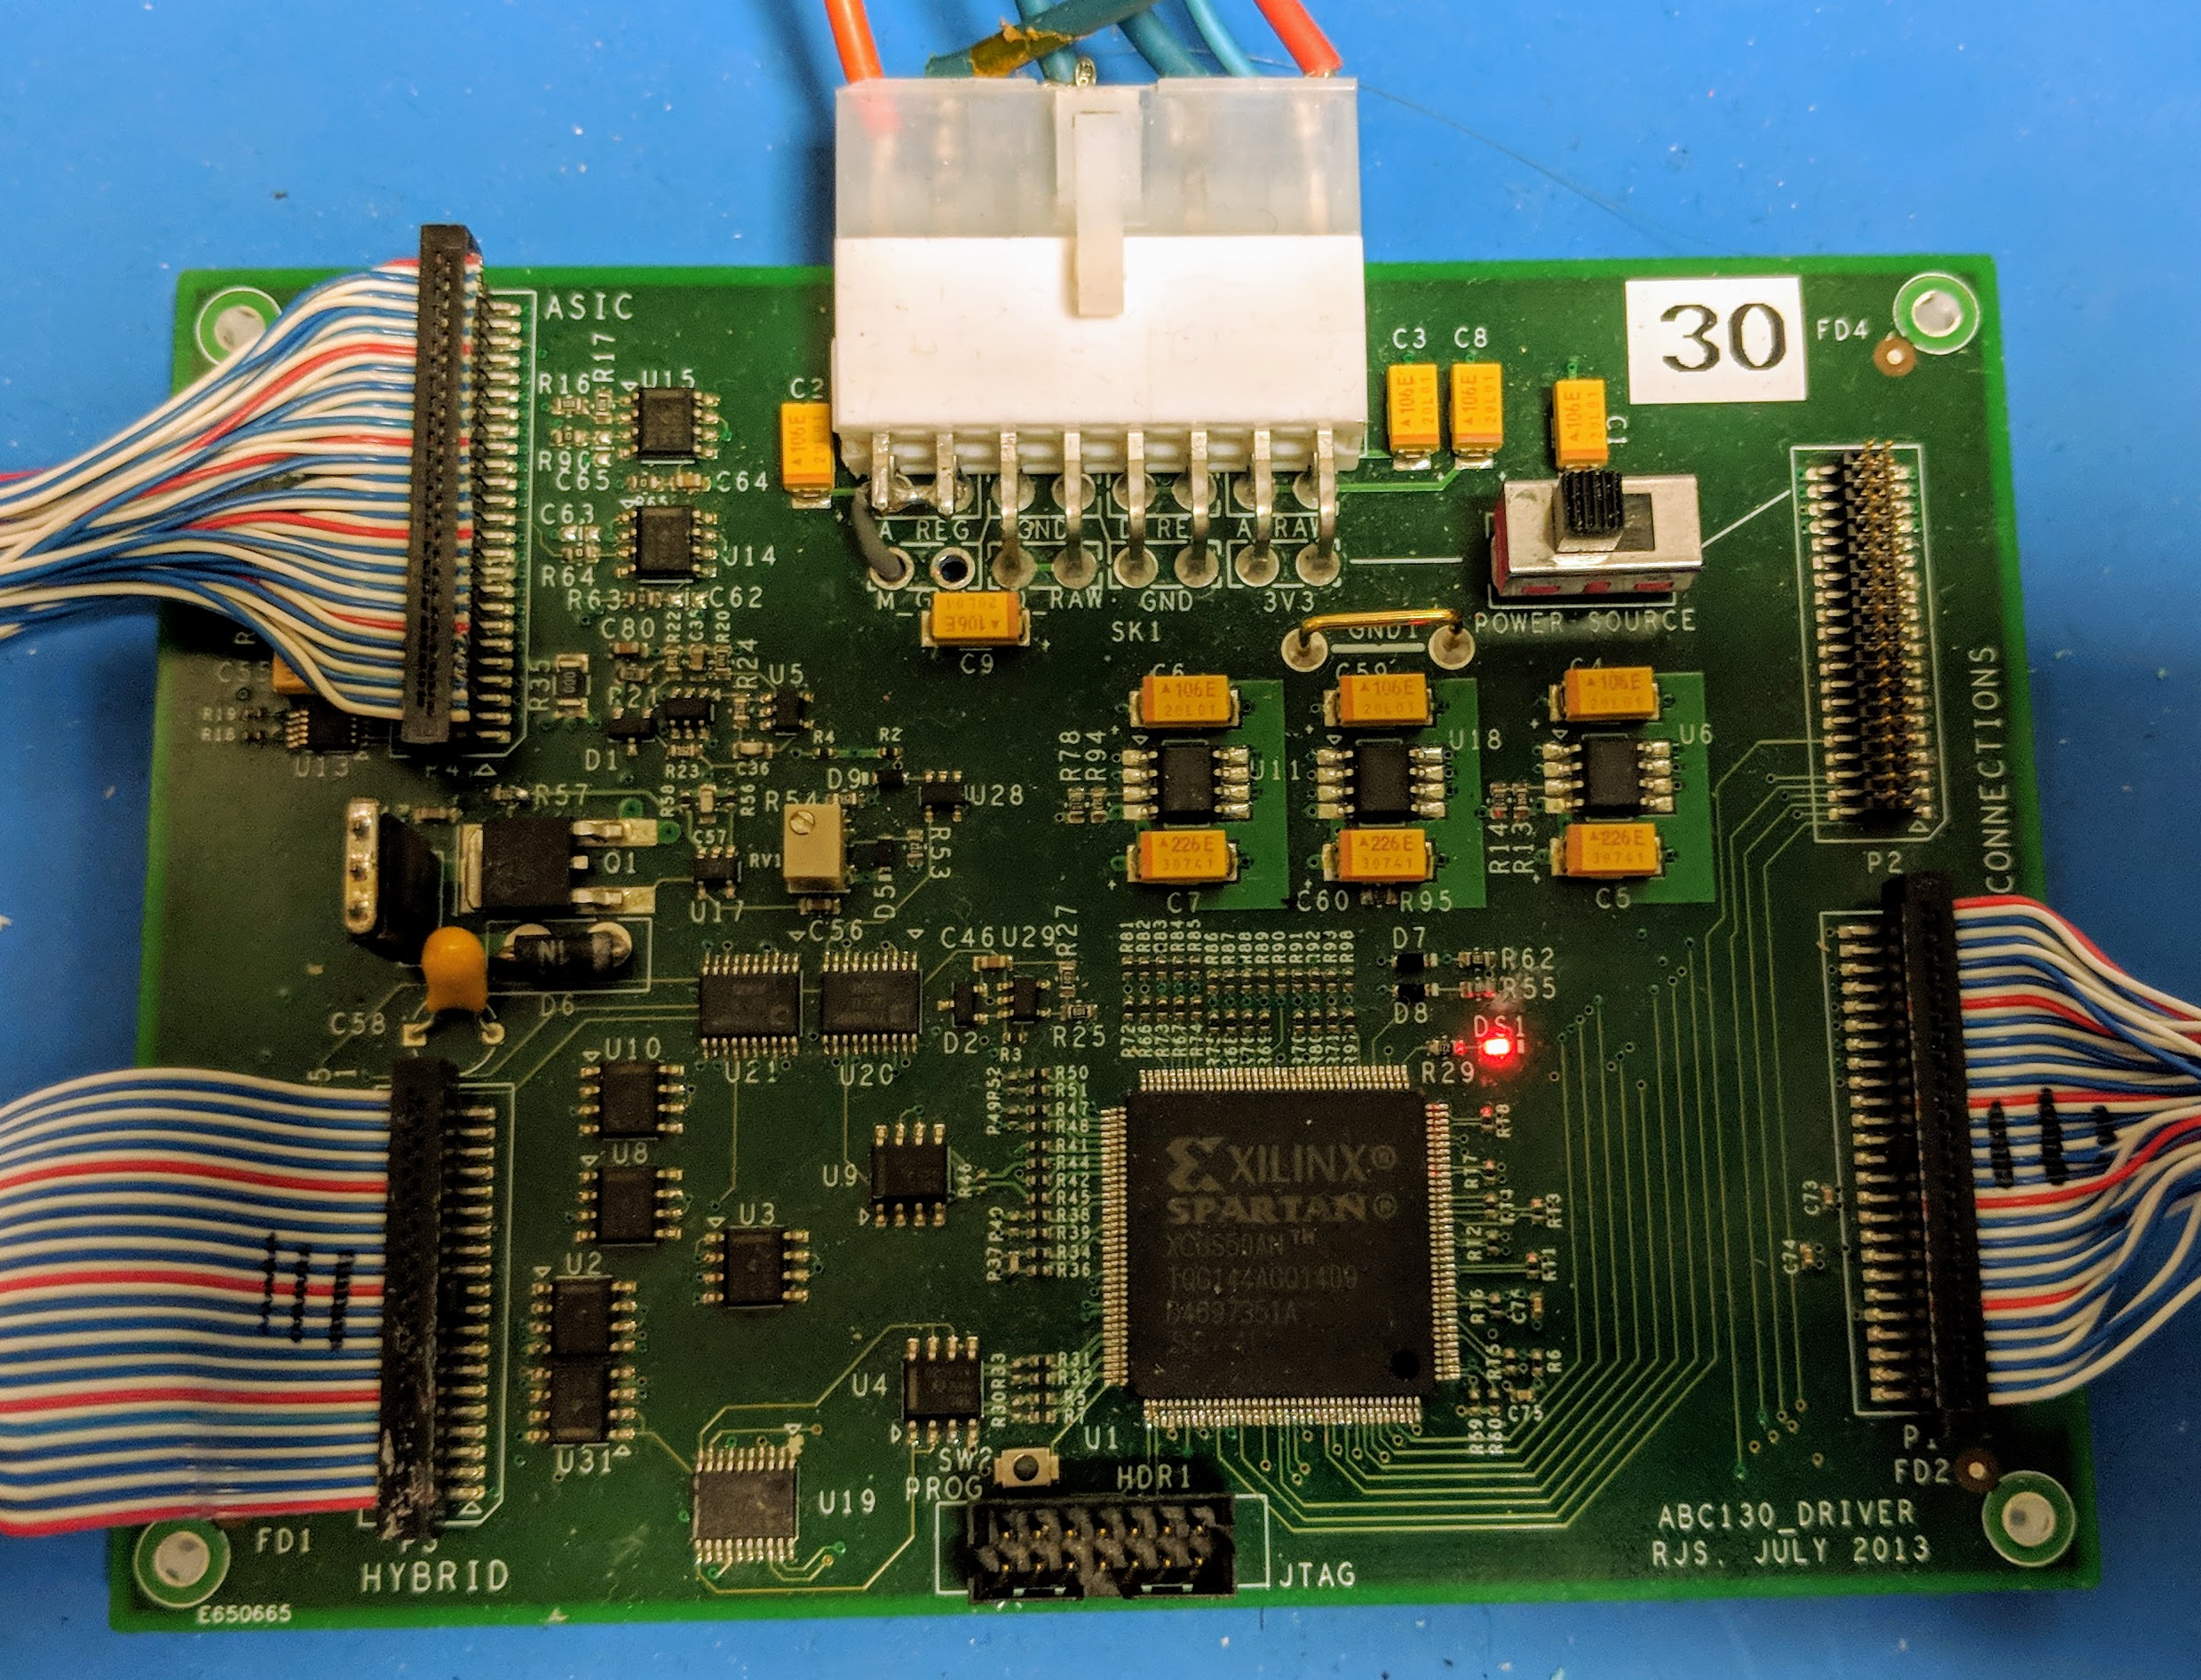
\includegraphics[width=0.8\textwidth]{images/hybrid_board.jpg}

            \column{0.3\textwidth}
            \begin{block}{}
                Orientation of the power, ABC130, and ATLYS connections.
            \end{block}
        \end{columns}
    }

    \frame{
        \frametitle{ABC130 Single Chip Test Card}
        \begin{columns}[c]
            \column{0.4\textwidth}
            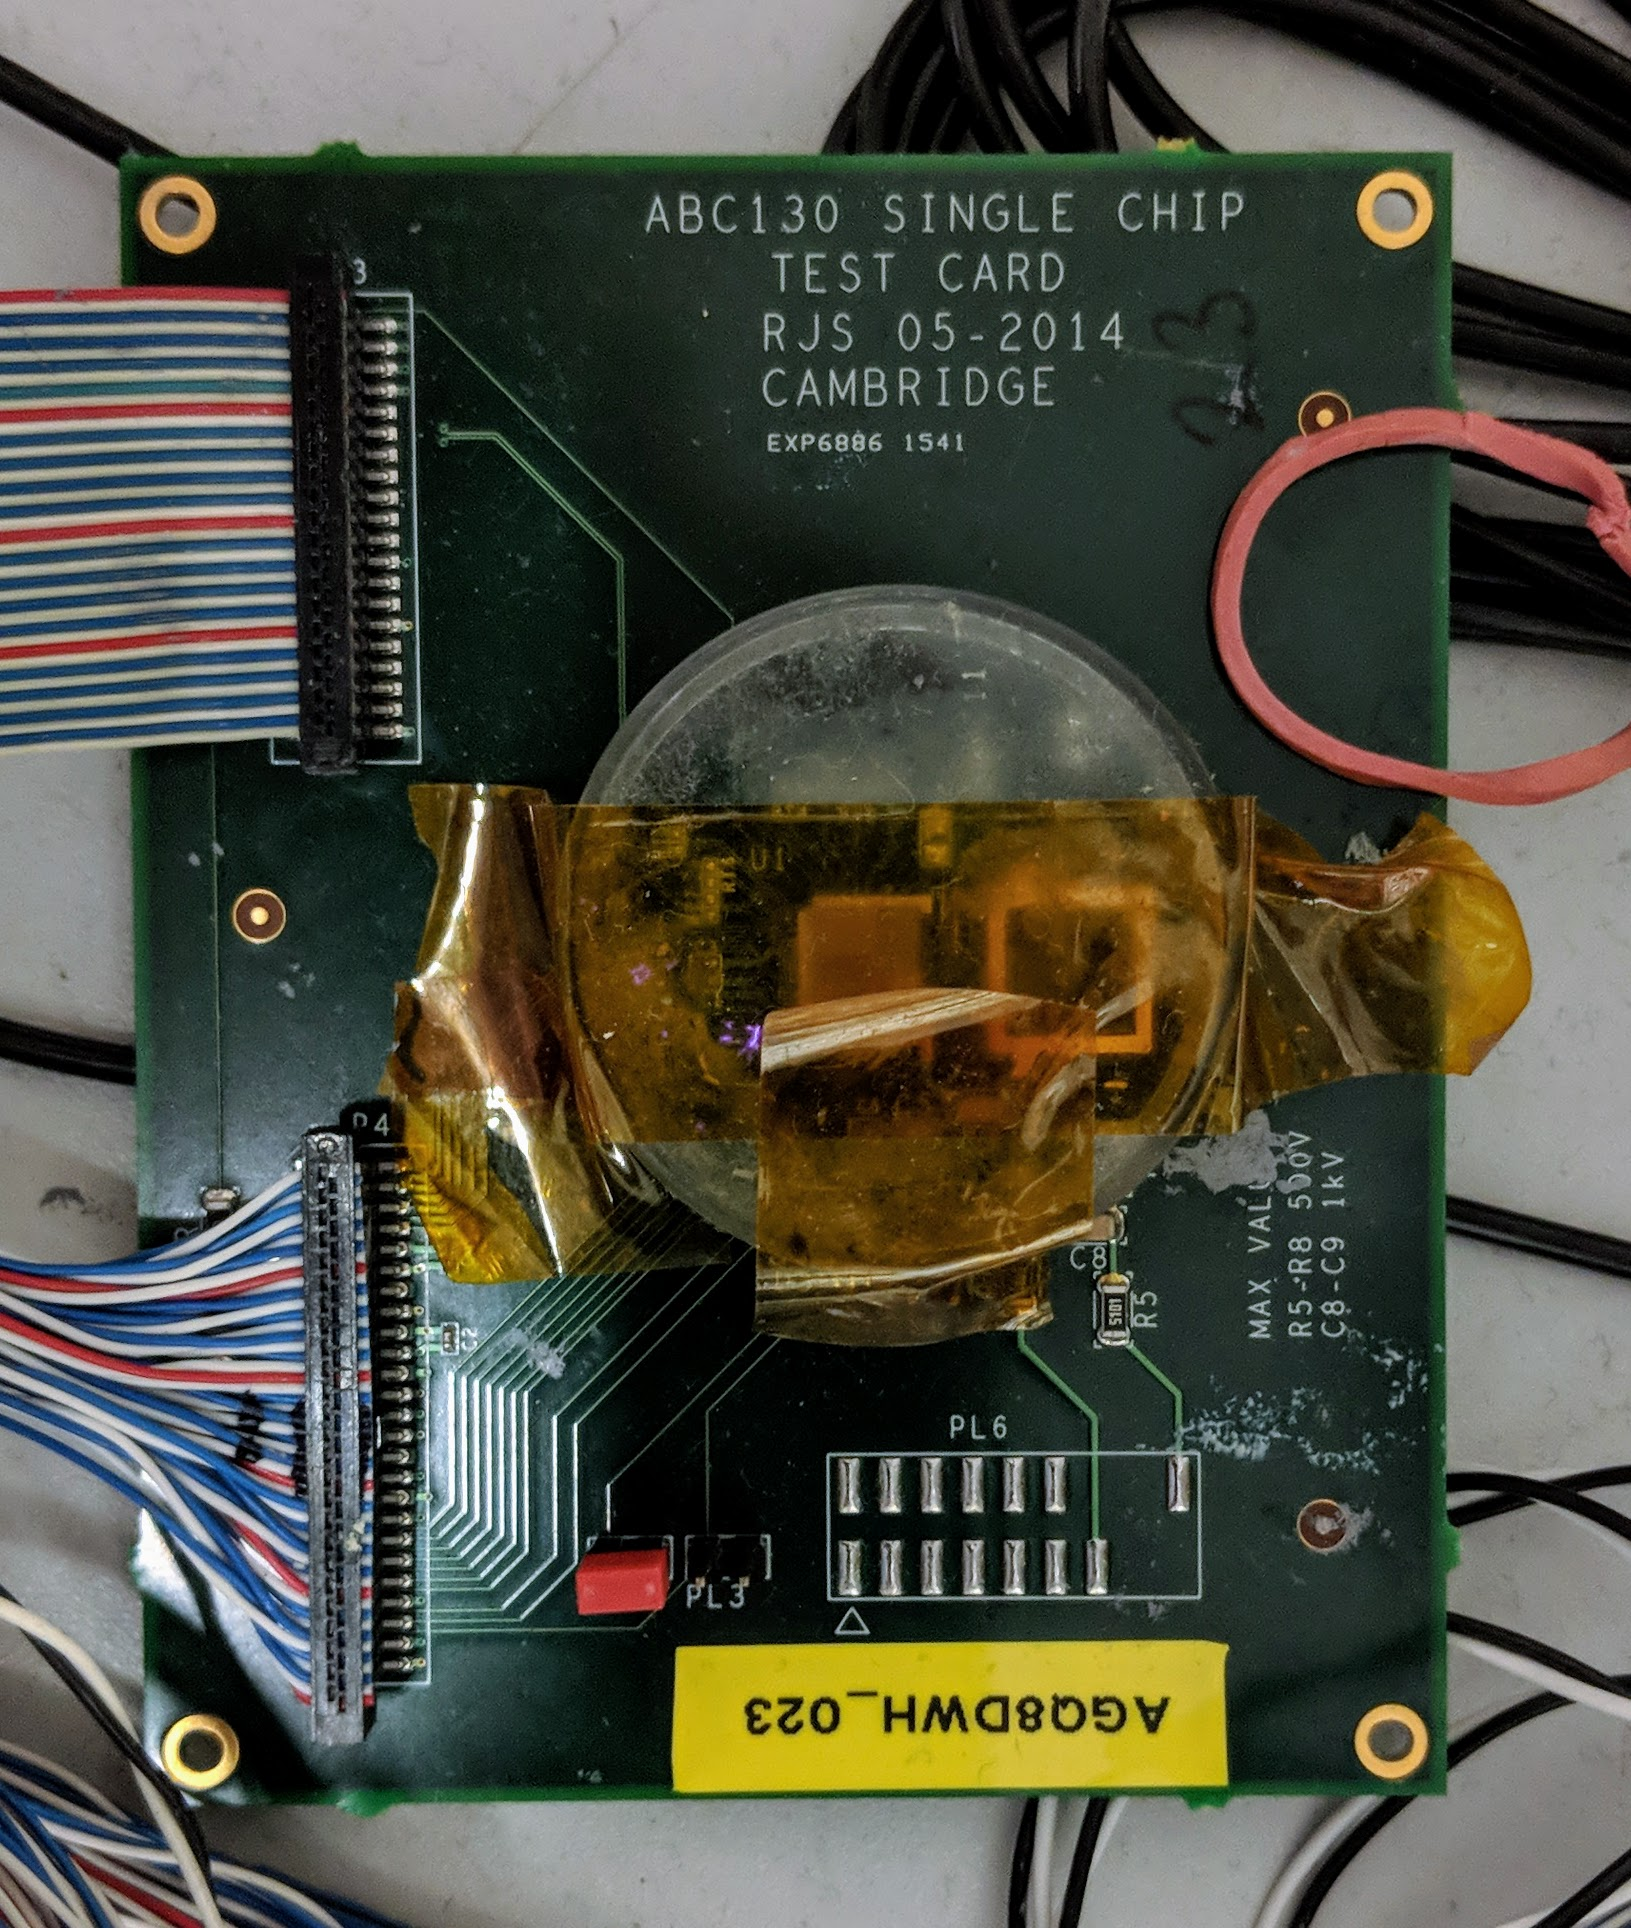
\includegraphics[width=1.0\textwidth]{images/ABC130_card.jpg}

            \column{0.6\textwidth}
            \begin{block}{}
                Test card, with connection to the driver board.
            \end{block}
        \end{columns}
    }

    \frame{
        \frametitle{The Hybrid Setup}
        \begin{columns}[c]
            \column{0.2\textwidth}
            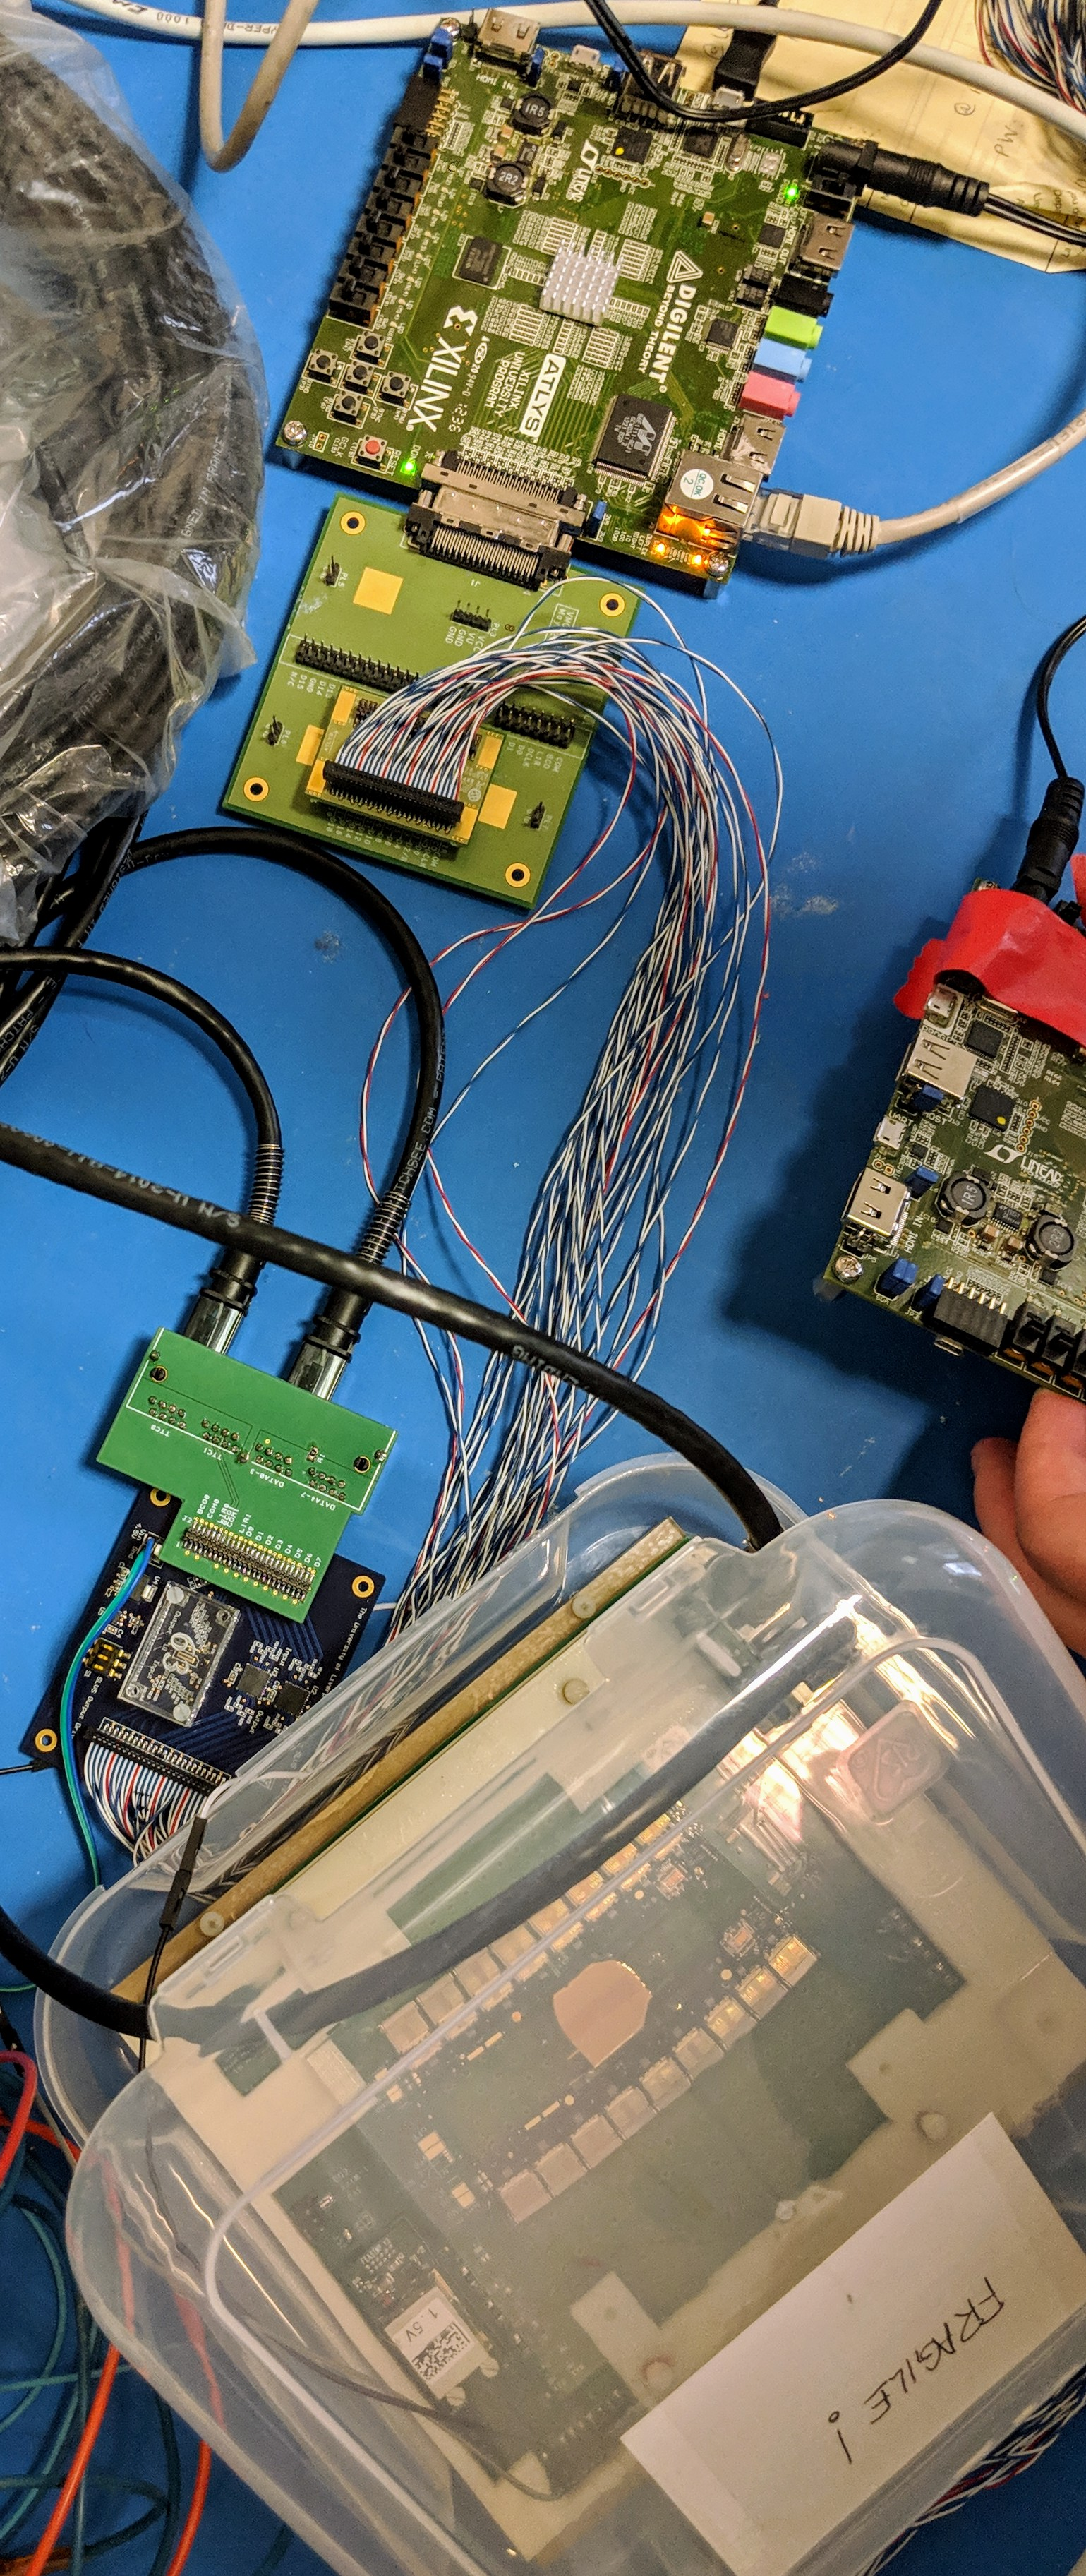
\includegraphics[width=1.0\textwidth]{images/hybrid_setup.jpg}

            \column{0.6\textwidth}
            \begin{block}{}
                The fully assembled readout chain for the hybrid chip.
            \end{block}
        \end{columns}
    }

    \frame{
        \frametitle{The Hybrid's ATLYS}
        \begin{columns}[c]
            \column{0.5\textwidth}
            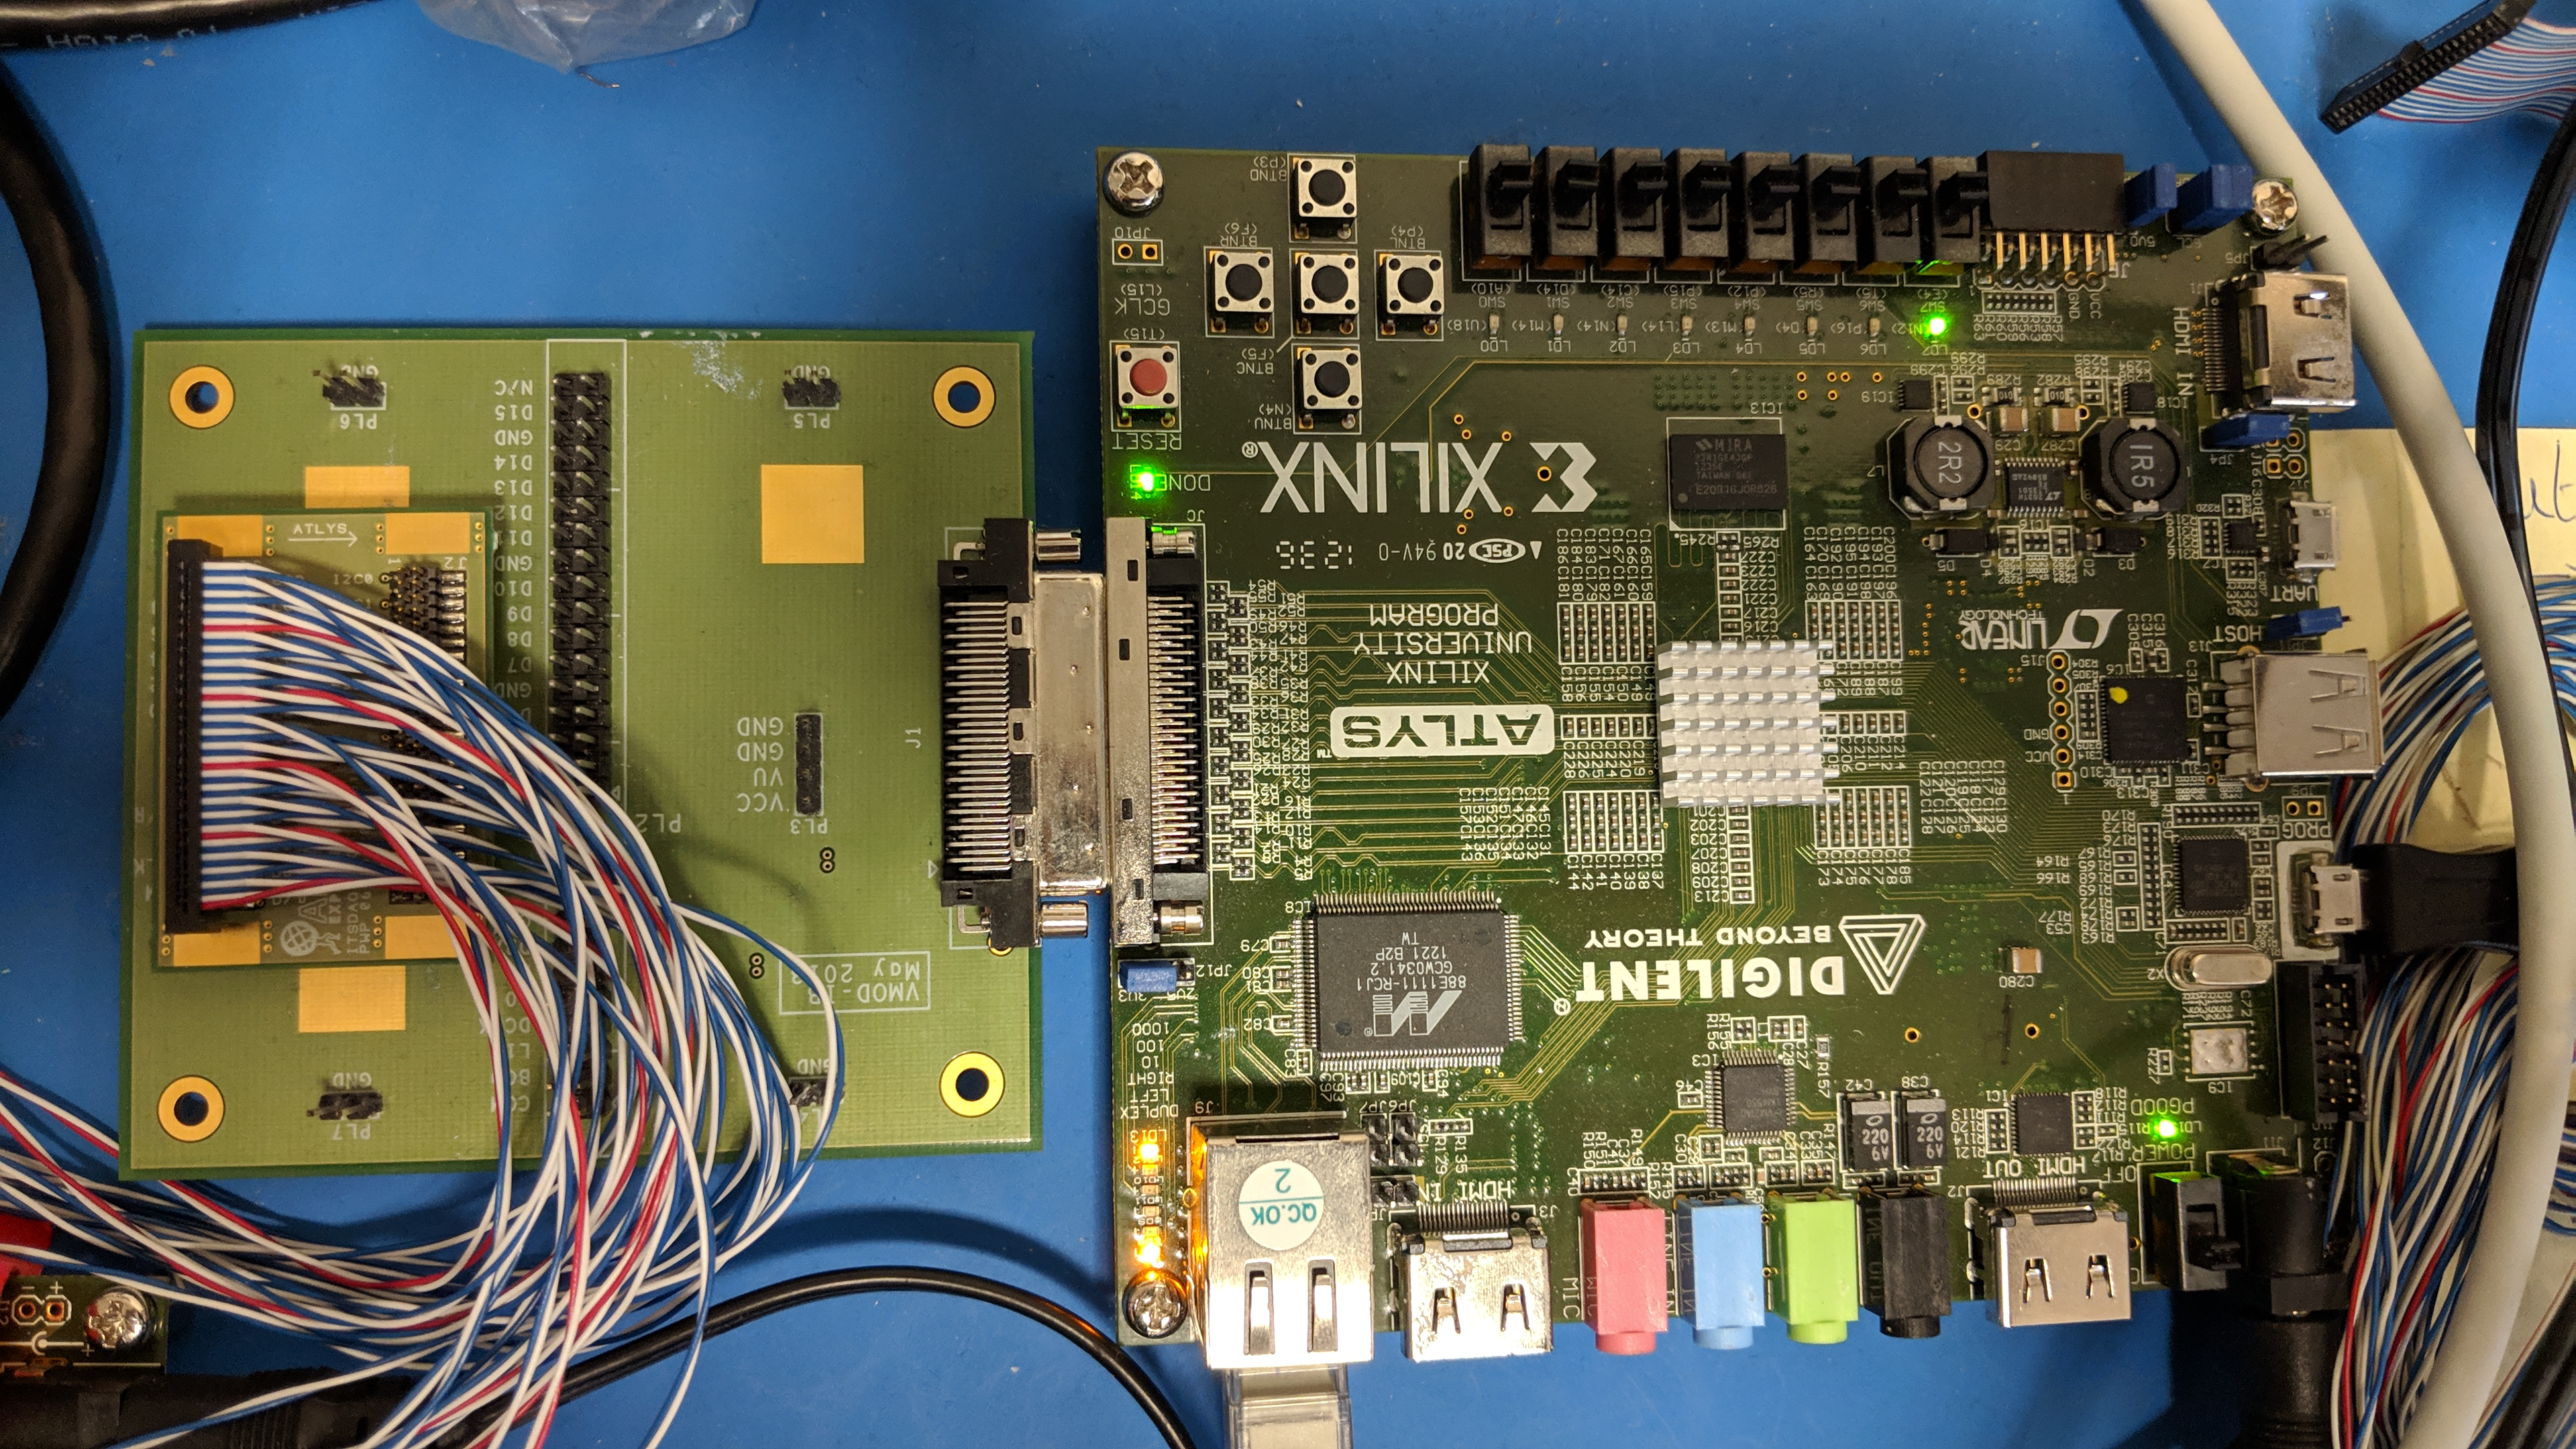
\includegraphics[width=1.0\textwidth]{images/hybrid_VMOD.jpg}

            \column{0.6\textwidth}
            \begin{block}{}
                Another VMOD-IB connection to another ATLYS.
            \end{block}
        \end{columns}
    }

    \frame{
        \frametitle{The Hybrid Driver Board}
        \begin{columns}[c]
            \column{0.5\textwidth}
            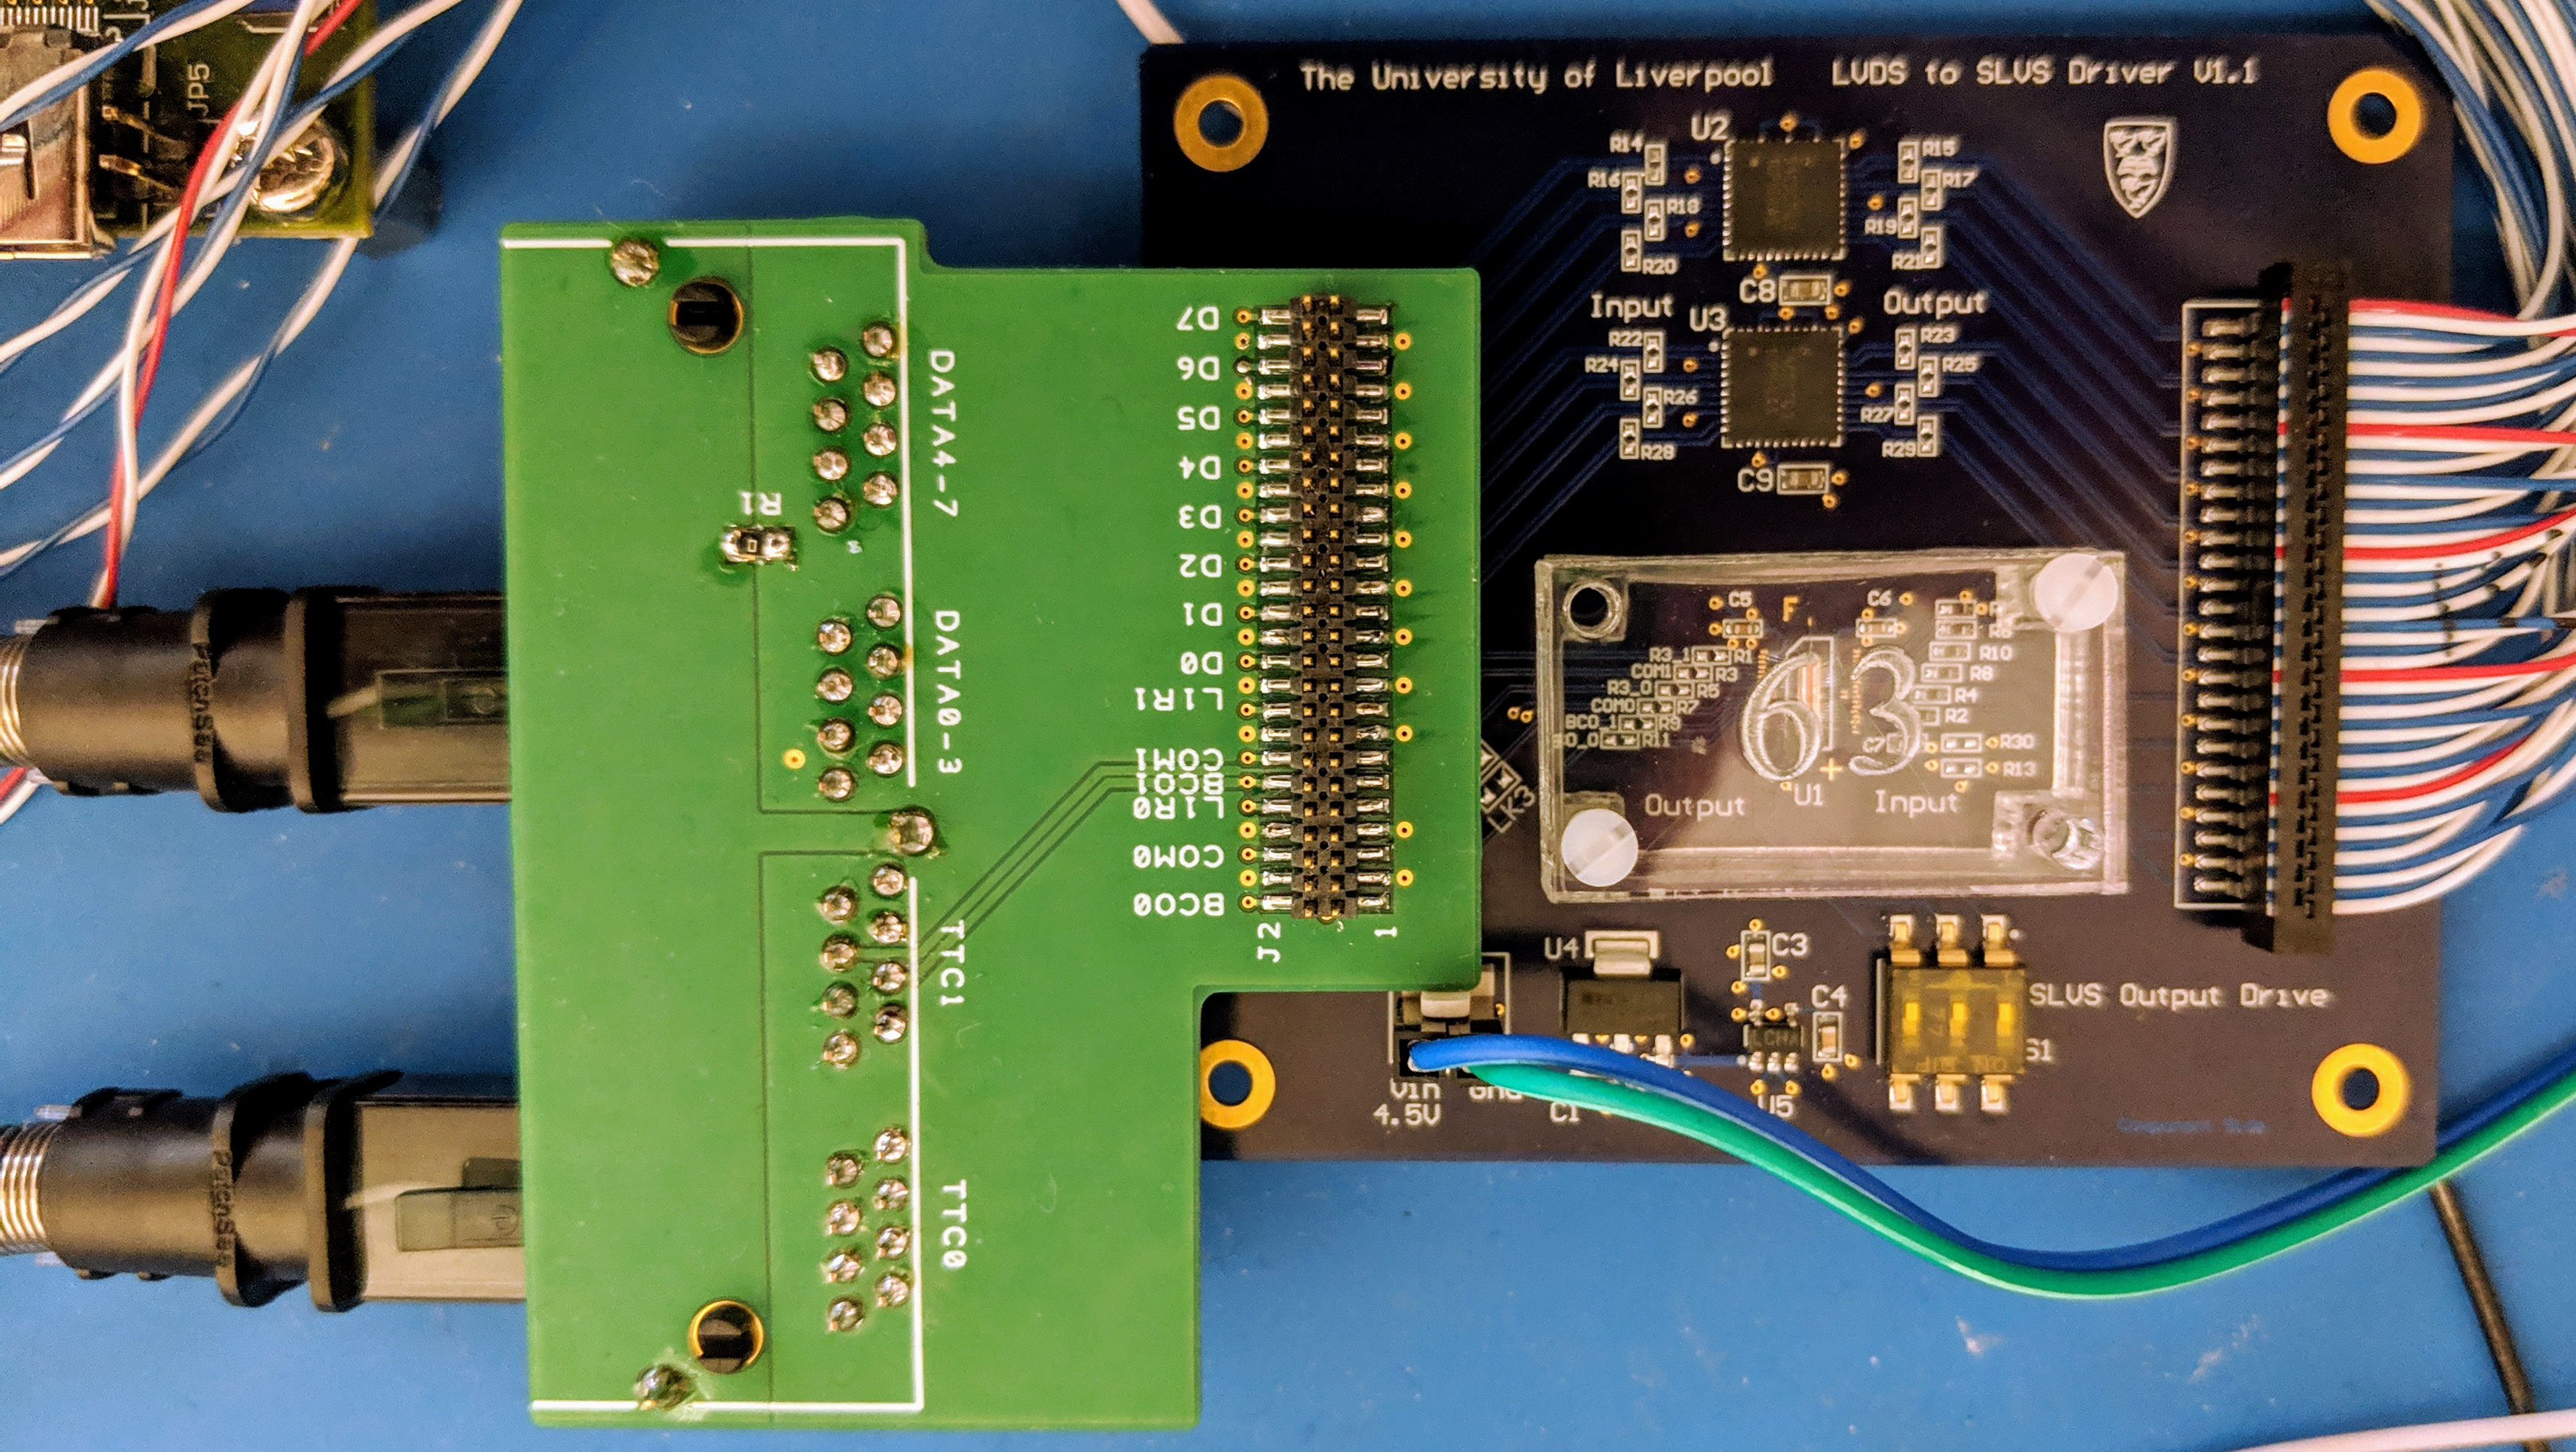
\includegraphics[width=1.0\textwidth]{images/hybrid_driver_board.jpg}

            \column{0.6\textwidth}
            \begin{block}{}
                LVDS to SLVS driver board.
            \end{block}
        \end{columns}
    }

    \frame{
        \frametitle{The Actual Hybrid Chip}
        \begin{columns}[c]
            \column{0.5\textwidth}
            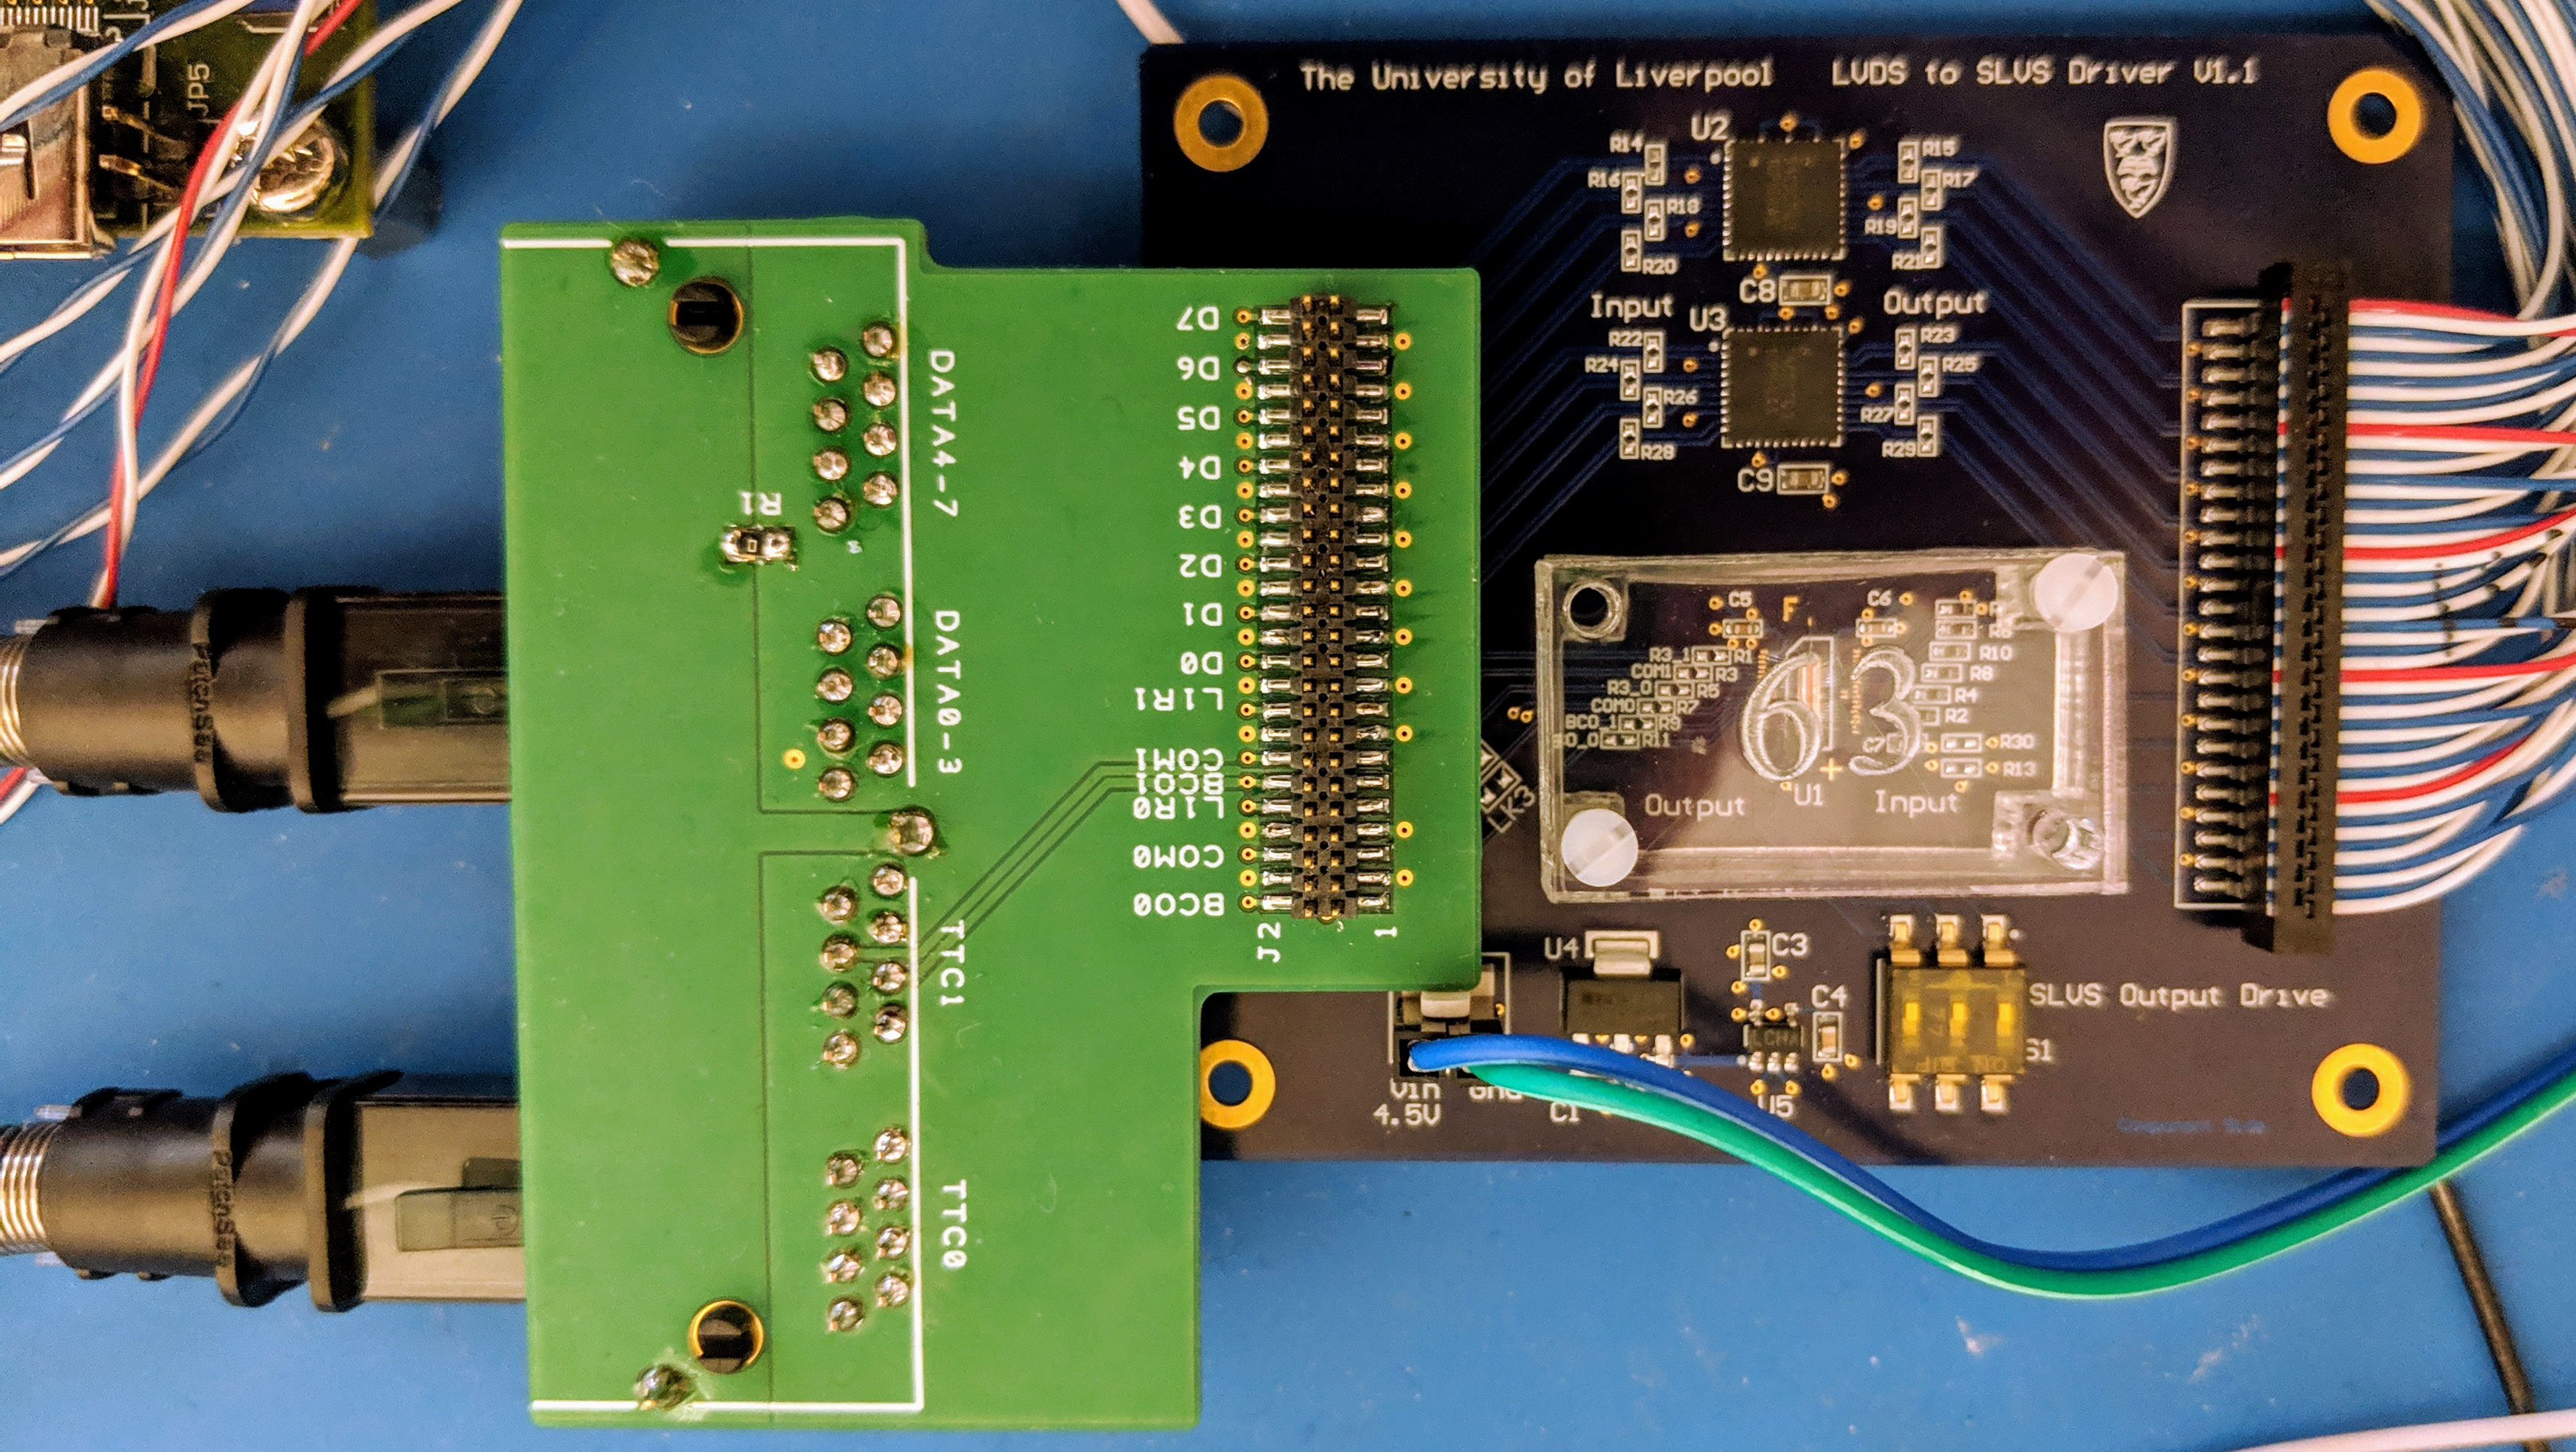
\includegraphics[width=1.0\textwidth]{images/hybrid_driver_board.jpg}

            \column{0.6\textwidth}
            \begin{block}{}
                The hybrid chip.
            \end{block}
        \end{columns}
    }

    \subsection{Progress \& Goals}

    \frame{
      \frametitle{Progress \& Obstacles}
      \begin{block}{Progress}
        \begin{itemize}
            \item Able to run correct versions of NI-VISA, NI-DAQMX Base, and NI-488.2 and communicate with devices
            \item Able to use the ITSDAQ software to run tests on actual chips
            \item Resolved 3-point voltage gain problem
        \end{itemize}
      \end{block}
      \begin{block}{Obstacles}
        \begin{itemize}
            \item The cabling connections to both the power supply and the ABC chips have been very sensitive
            \item Firmware issues with the on the ATLYS connected to the hybrid chip
        \end{itemize}
      \end{block}
    }

    \frame{
      \frametitle{3 Point Gain Not Working}
      Measures gain \& noise at 3 power supply currents
				\begin{figure}
					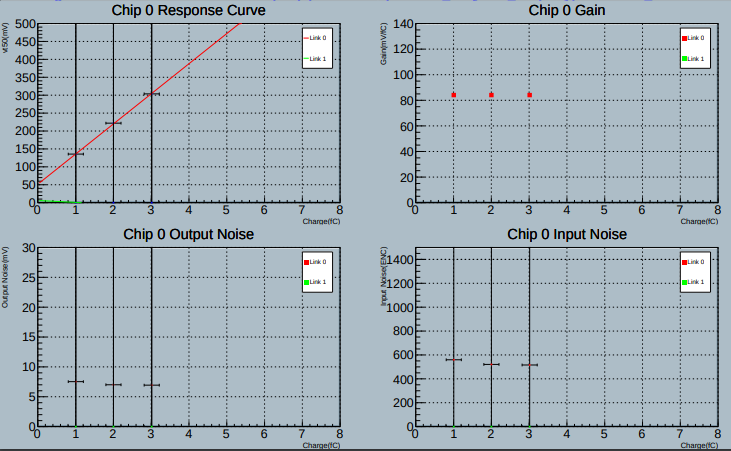
\includegraphics[trim={0cm 0cm 0cm 0cm},clip,width=0.5\textwidth]{images/3pg1.png}
				\end{figure}

    }
    \frame{
      \frametitle{3 Point Gain Not Working}
      Measures gain \& noise at 3 power supply currents
				\begin{figure}
					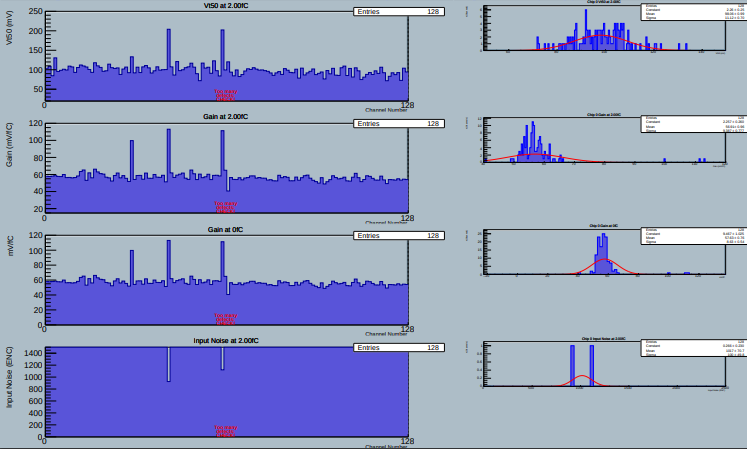
\includegraphics[trim={0cm 0cm 0cm 0cm},clip,width=0.5\textwidth]{images/3pg2.png}
				\end{figure}

    }

    \frame{
      \frametitle{3 Point Gain Working}
      Measures gain \& noise at 3 power supply currents
				\begin{figure}
					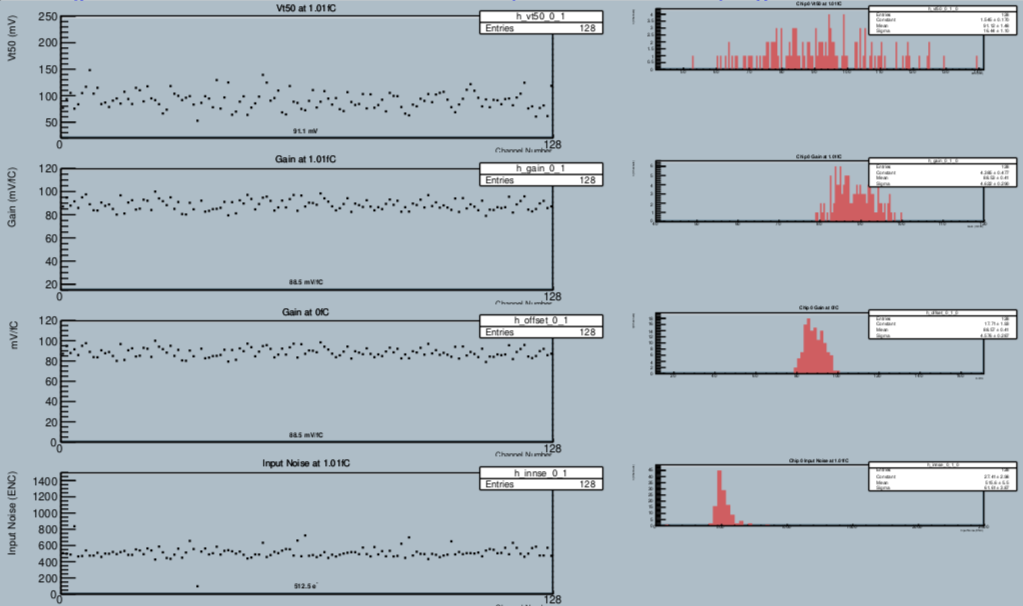
\includegraphics[trim={0cm 0cm 0cm 0cm},clip,width=0.5\textwidth]{images/good_noise.png}
				\end{figure}

    }
    \frame{
      \frametitle{3 Point Gain Working}
      Measures gain \& noise at 3 power supply currents
				\begin{figure}
					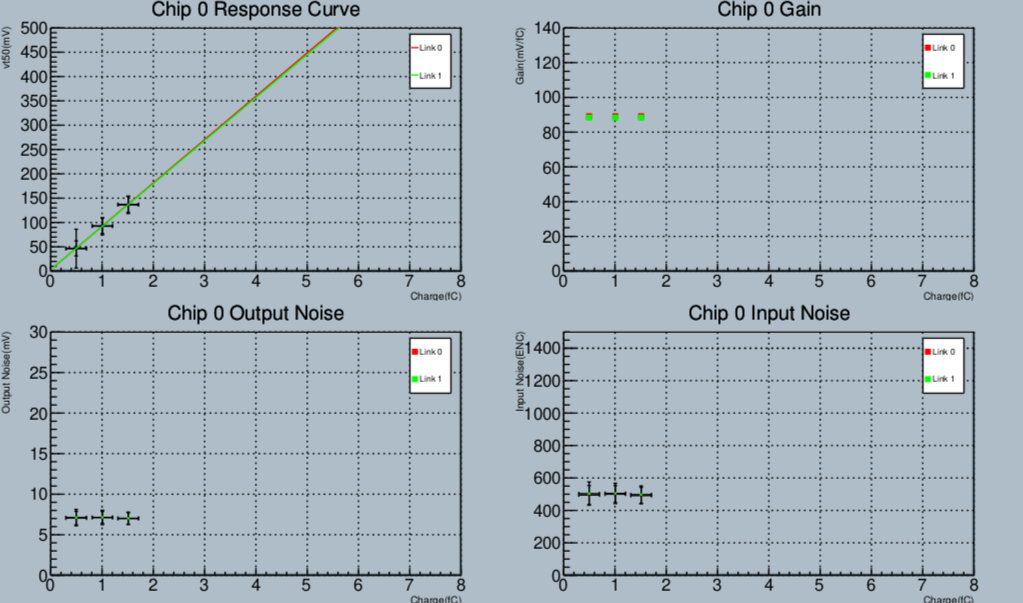
\includegraphics[trim={0cm 0cm 0cm 0cm},clip,width=0.5\textwidth]{images/good_3PG.png}
				\end{figure}

    }

    \frame{
      \frametitle{Goals}
      \begin{block}{}
        \begin{itemize}
            \item Resolve ATLYS hybrid firmware issues
            \item Obtain a stable cabling setup
            \item Integrate FELIX chip (optical, rad-hardened comm protocol drivers) into readout chain
        \end{itemize}
      \end{block}
    }


    % ============================================================== %
    %
    % Acknowledgements
    %
    % ============================================================== %

    \section{Acknowledgements}


    \frame{
        \frametitle{Acknowledgements}

       \begin{minipage}{\textwidth}
        We would like to acknowledge the University of Michigan Department of Physics,\\
        specifically Jean Krisch, Tom Schwarz, and Steven Goldfarb.
        We would also like to acknowledge the support of the Lounsbery foundation.   \\
       \end{minipage}


        \begin{minipage}{\textwidth}

          \begin{figure}
            \centering
            \begin{subfigure}
              \centering
               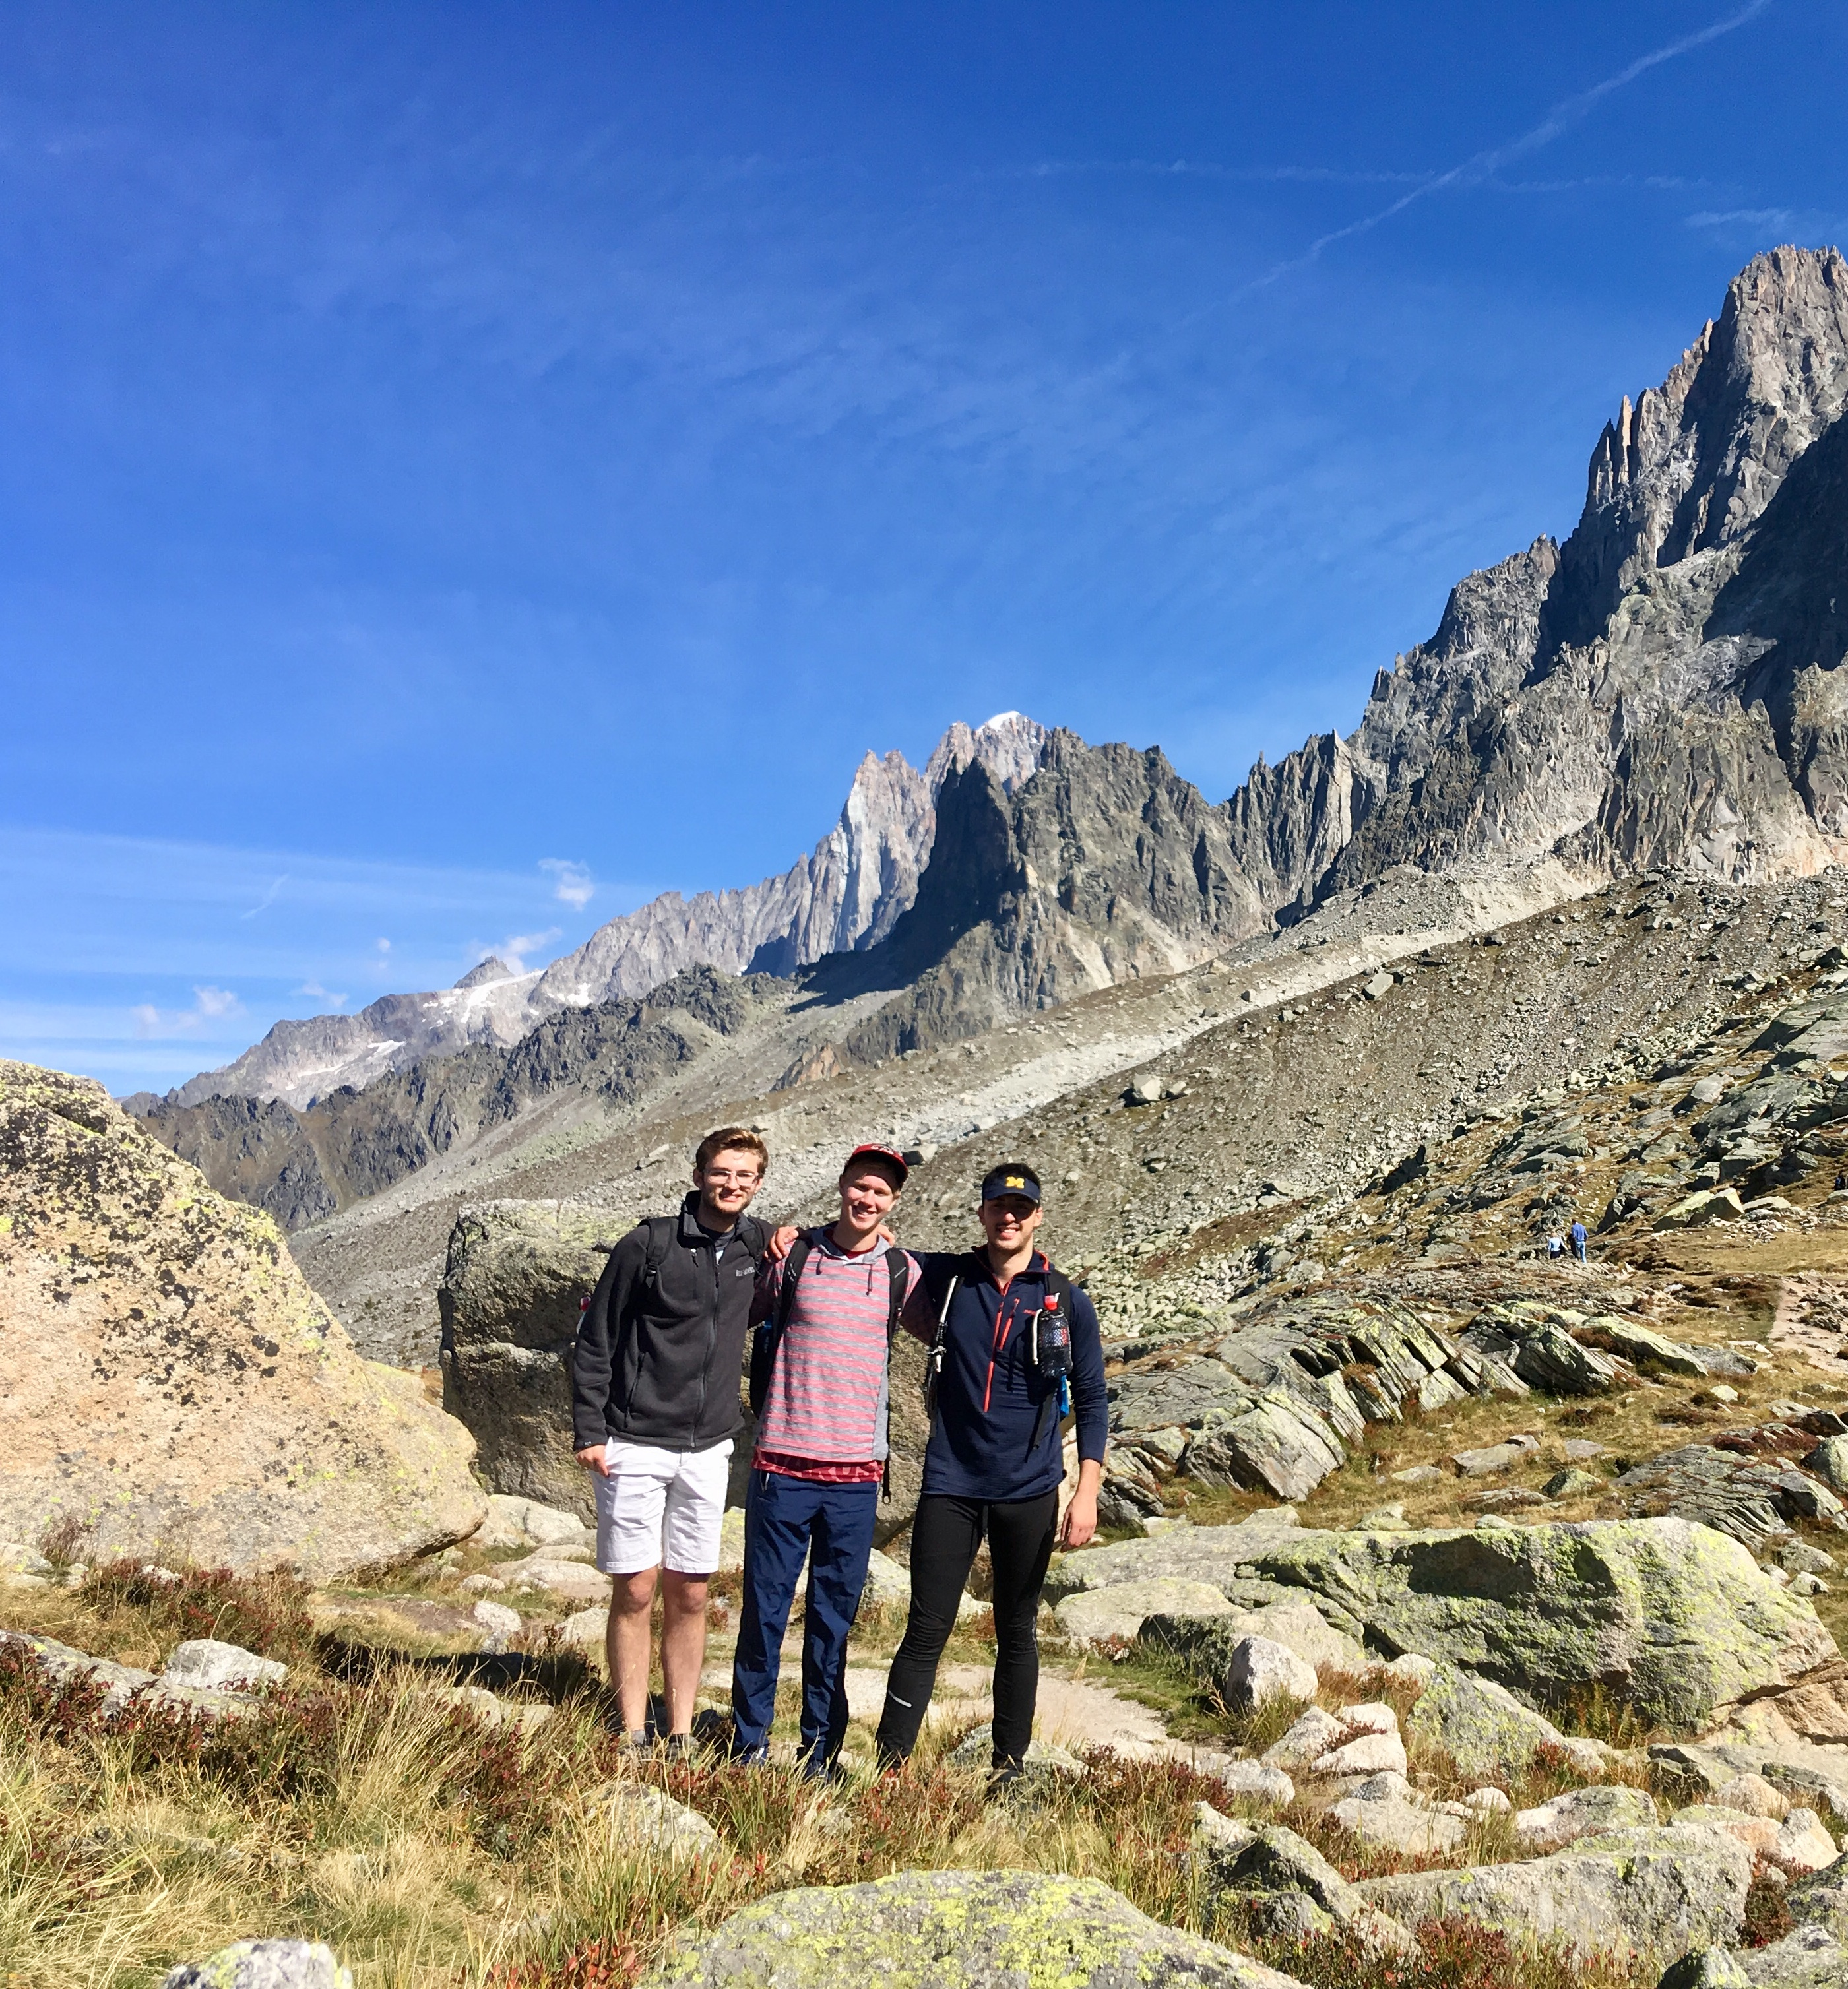
\includegraphics[scale=0.04,trim={0 0 0 35cm },clip]{p1-figs/cham.jpg}
            \end{subfigure}
            \begin{subfigure}
              \centering
              	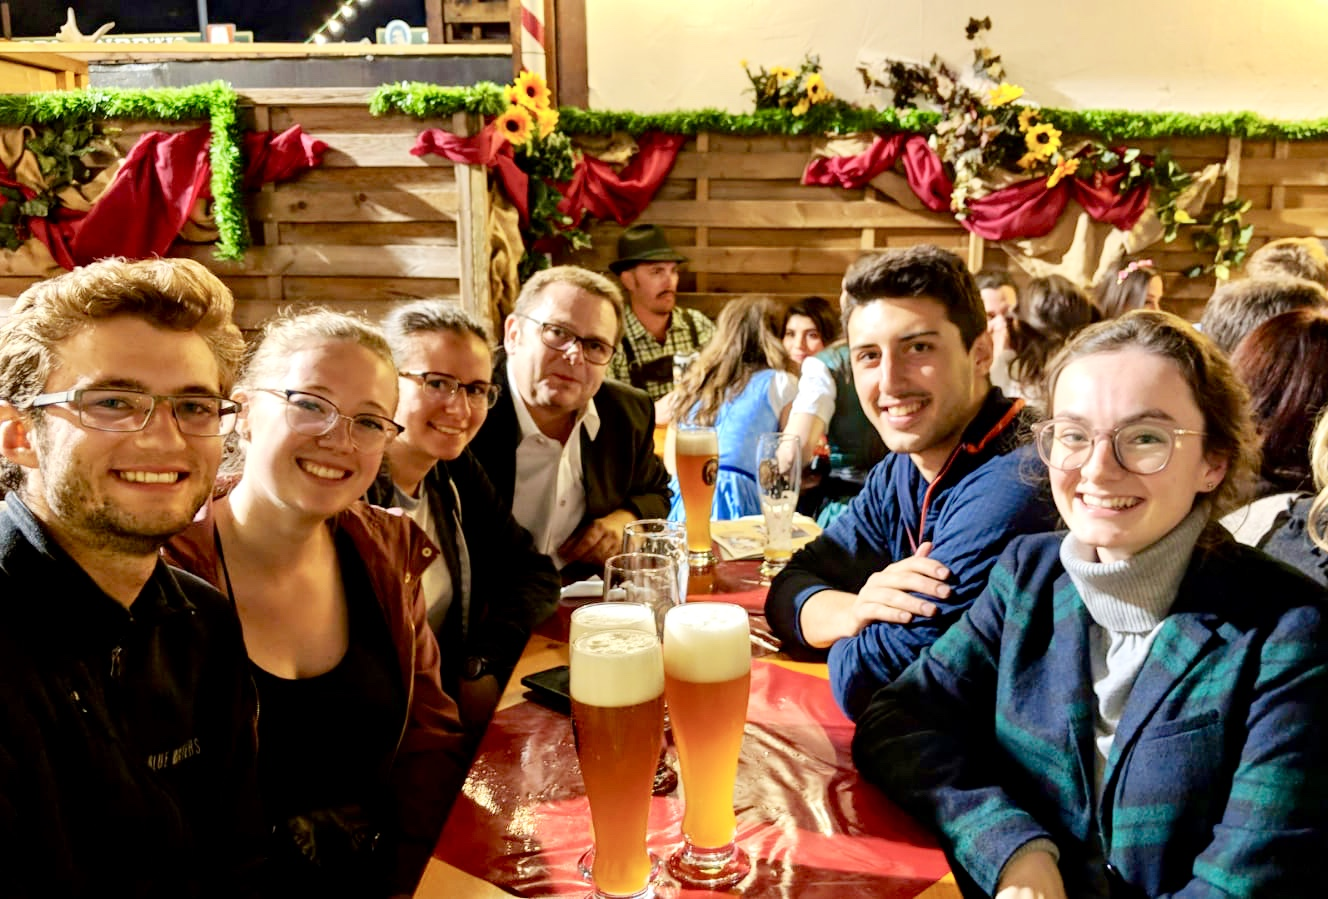
\includegraphics[width=0.25\paperwidth]{p1-figs/okto.jpg}
            \end{subfigure}
            \begin{subfigure}
              \centering
              	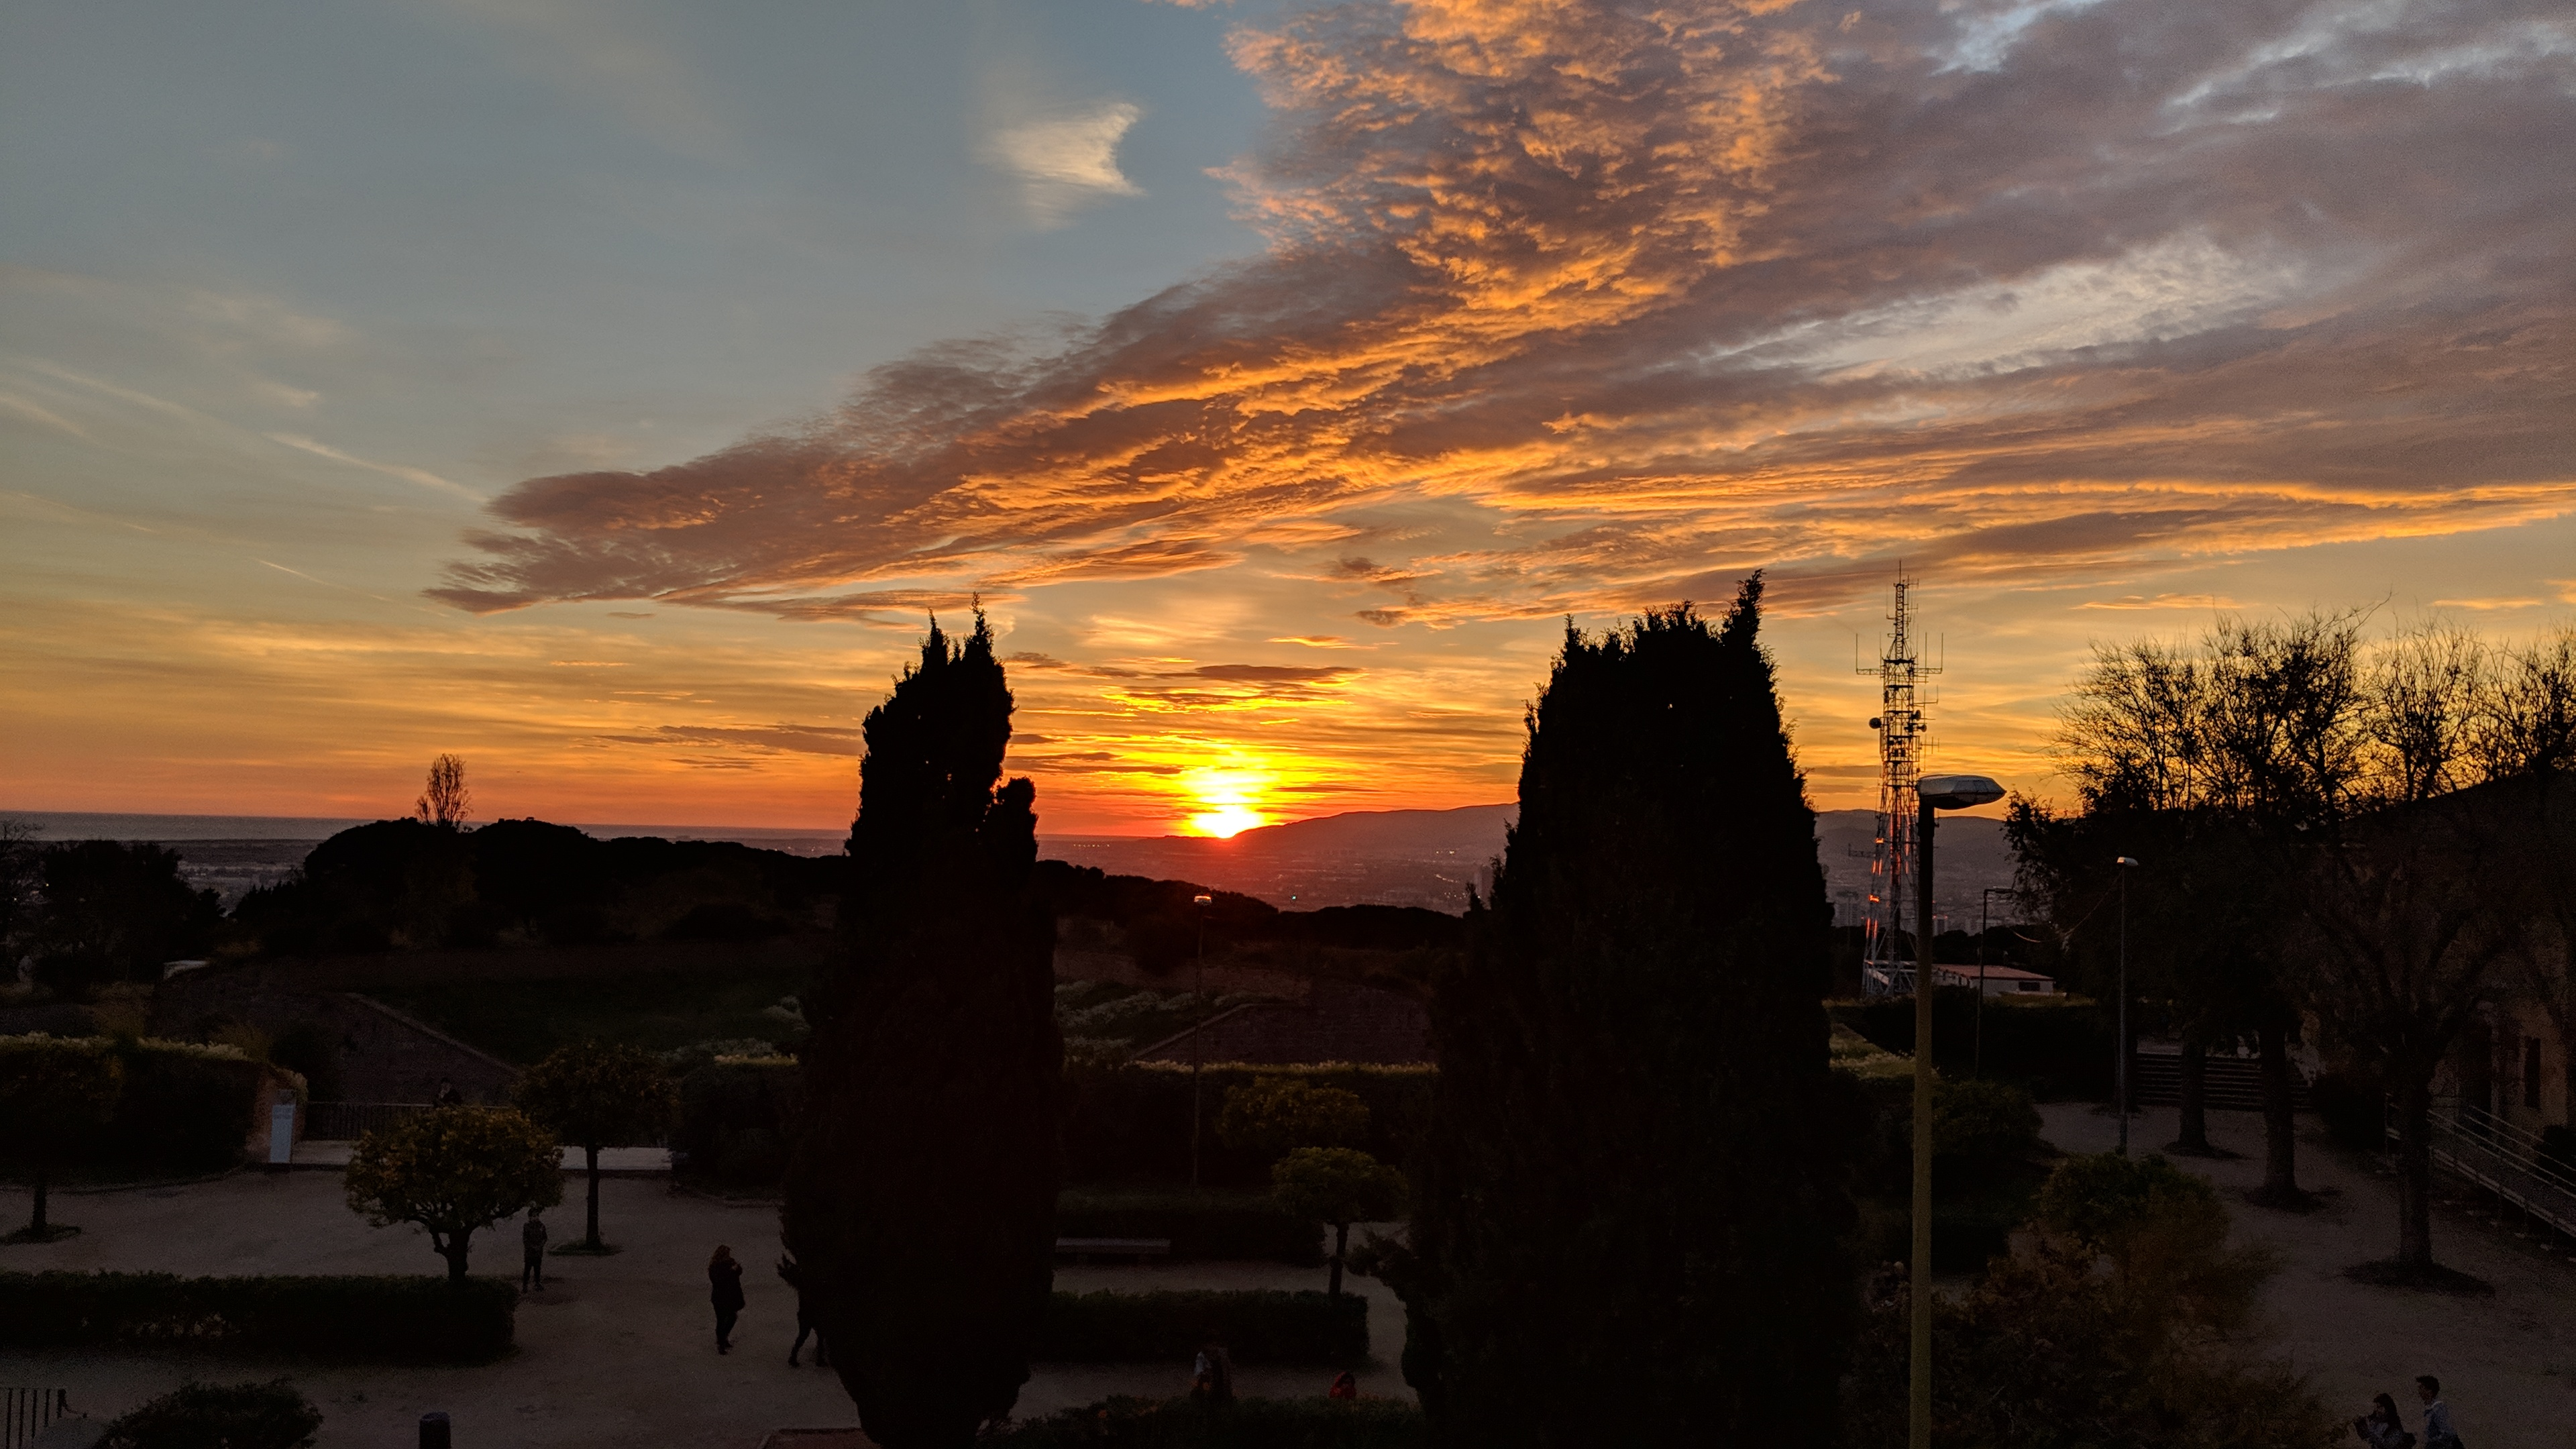
\includegraphics[width=0.30\paperwidth]{images/barcelona.jpg}
            \end{subfigure}
          \end{figure}
        \end{minipage}

    }

    \section{}
    \cernSplashWhite

\end{document}
